\documentclass{article}
\usepackage{graphicx} % Required for inserting images
%\usepackage{geometry}
%\geometry{margin=0.5in}
%\usepackage{cite}
%\usepackage{color}

%\title{XMLTDB01}
%\author{Bo Sundman et al. }
%\date{June 2023}

\usepackage[utf8]{inputenc}
\usepackage{amssymb}
\usepackage{graphicx,subfigure}              % with figures
% sometimes needed to have pdf files 
\pdfsuppresswarningpagegroup=1
\topmargin -10mm
\oddsidemargin -10mm
\evensidemargin -10mm
\textwidth 170mm
\textheight 220mm
\parskip 2mm
\parindent 3mm
%\pagestyle{empty}
\usepackage{xcolor}
\usepackage[normalem]{ulem}

%footnote using capital letter
\renewcommand{\thefootnote}{\Alph{footnote}}
%\renewcommand{\thefootnote}{{\arabic{footnote}}

% For appendices
\usepackage[titletoc,title,header]{appendix}

\begin{document}

\begin{center}

  {\Large \bf Proposal 0.0.4 of an XML format to replace TDB files}

  Bo Sundman et al. \today

  \vspace{5mm}

  {\large \bf Background}

\end{center}

\bigskip

The current TDB format for Calphad databases has worked well for 40
years but introducing new models and features has revealed some
awkward features, in particular the TYPE\_DEFINITION keyword.  When a
change is needed it may be interesting to adopt an accepted Markup
Language as XML or JSON.  The XML has been selected for a new XTDB
format as it has been around for a long time and is slightly more
explicit.

There are many Markup Languages but as it is easy to convert between
them the choice of XML is not very important except to avoid spending
a year or two to discuss this choice.

XML is flexible and extendable each software may add their own flavour
in a controlled way.  It will be simpler to use an XTDB file by
different softwares as one can easily indicate what is software
specific rather than try to modify or extend the TDB format.

In section~\ref{sec:changes} the most important changes from previous
versions of this proposal are listed and motivated.

To avoid the confusing use of {\bf ELEMENT} both for chemical element
and the XML element I now use {\bf TAG} for the XML element.

The proposal here is a minimal change from the TDB format intended to:
\begin{itemize}
  \item make manually editing an XTDB file as easy as the current TDB
    format.
  \item minimize problems when using software A to read a database
    file written by software B.
  \item provide better facilities to handle new models and features
    added by the different softwares using Calphad databases.
  \item provide users of a database with information about the
    bibliographic information even for encrypted databases.
  \item Software will be able to add tags and attributes in the
    database with minimal problems when the database is read by other
    software.  Such modifications should not affect the thermodynamic
    data itself.  Significant new features should be discussed with
    SGTE and integrated in the XTDB format.
\end{itemize}

This XTDB definition may require minor modifications in the XML format
already adoped in some software.  Commercial companies providing
encrypted databases to customers can use whatever format they prefer
for such databases.  But they should provide a facility to read and
write unencrypted databases in the XTDB format.

You are encouraged to ask anyone you think can contribute to defining
the new database format to have a look at this and provide their
comments.

\newpage

\section{How this document can be read}

The following proposal is for a common definition of an XTDB file
format based on XML.  It can hopefully become an SGTE standard
acceptable by all software which develop or use Calphad databases.

If you already read an earlier version of this maybe look at the next
section and the examples in the Appendix to see if anything changed.
Then look at points to discuss in section~\ref{sec:points}.  If you
find all OK or have some questions or comments send a message to
bo.sundman@gmail.com to explain your points of view.

If you read the XML tag definitions in sections~\ref{sec:first} to
\ref{sec:soft} and the corresponding notes please note what you like
or dislike and send a message to to bo.sundman@gmail.com to explain
your points of view.

If you are not familiar with XML there are plenty of information
online.  In brief XML has ``tags'' with ``attributes''.  The tags and
attributes proposed for the XTDB format are listed in the sections
below and the attributes are explaines and may have a ``note''.  If
the note is ``+'' the attribute is compulsory, ``--'' if optional.  A
letter A-Z in the note referes to details explained in
section~\ref{sec:notes}.

In this document a tag is usually in {\bf bold} when refereced in the
text and an attribute in {\em italics}.  But I have not been totally
consequent.  All values of the {\em Id} attributes are case
insensitive as in the TDB file.  Except for phase names the value of
an {\em Id} cannot be abbreviated when used in other attributes.

An XML parser is convenient for reading XML files but to simplify the
life for all the the humans reading and editing the XTDB file it is
strongly recommended that the attributes to an XML tag are provided in
the order listed for each tag below.  Software specific attributes can
be added to a tag but should come at the end.

The order of XML tags in the XTDB file is fairly free but to
simplify for a human reader and editing the XTDB file a recommended
order is {\bf Defaults, DatabaseInfo} followed by {\bf Element,
  Species} and {\bf TPfun}s, {\bf Phases} (with many nested tags).
These will be followed by {\bf Parameter}s, ordered by phases or {\bf
  System} and finally the {\bf Bibliography}.  Optionally the {\bf
  Model} tag and {\bf AssessedSystem} and other tags at the end.

As a rule a tag or attribute starts with a capital letter and if it
consists of two or more parts, such as {\em NumberOf}, the second part
is joined without hyphen or underscore but starts also with a capital
letter.

\subsection{Significant changes from earlier versions}\label{sec:changes}

\begin{enumerate}
\item The ``DISORDERED\_PART'' which can occur in the TYPE\_DEFINITION
  in TDB files for some phases is now called {\bf DisorderedPart}.  I
  have previously called it SplitPhase.

\item The {\bf Constituent} tsg inside the {\bf Parameter2} tag is
  changed to {\bf SublConst} to avoid confusing with the {\bf
    Constituents} tag used inside the {\bf Phase} tag.

\item The FCC4PERM and BCC4PERM are models in the {\bf Permutations}
  tag.

\item Two complete examples added for Al-C with new unaries from Malin
  and Al-Li from Bengt with a suggestion for a CrystalStructure tag
  and 2 variants of the {\bf DisorderedPart} tag with and without the
  {\rm Disordered} attribute for the ordered FCC and BCC phases.

\item I have tried to update every part of this text when there has
  been suggestions I find interesting and useful. {\bf But it means
    there can be inconsistencies between different parts of this
    document.}

\item Some new tags introduced such as {\bf AppendiXTDB} and {\bf
  CrystalStructure}.  The {\bf AssessedSystem} tag is removed and
  replaced by several {\bf xSystem} tag.

\item I have merged the {\bf System} and {\bf AssessedSystem} tags and
  replaced them by {\bf UnarySystem}, {\bf BinarySystem} and {\bf
    TernarySystem} tags, including an optional {\em Command} attribute
  to calculate a diagram.  An optional {\em Command} attribute (which
  requite there is a {\em Software} attribute in the {\bf Defaults}
  tag) provides a software specific way to calculate the phase
  diagram.

  A {\bf Parameter} tag can appear anywhere, it is optional to include
  those relevant within a {\bf BinarySystem} or {\bf TernarySystem}
  tag.  It is not an error to have a {\bf Parameter} for another
  system inside a {\bf xSystem} tag.

\item The attribute {\em Software} added to the {\bf Default} tag.
  
\end{enumerate}

\subsection{UPPER and lower case and abbreviations}

In a TDB file UPPER and lower case letters was treated as identical.
The XML tags and attributes are case sensitive.  But I propose that in
the attribute values, for example elemen, species and phase names, the
UPPER and lower case letters will be considered as identical.

I prefer not to allow the characters ``(`` and ``)'' in the {\em Id}
attribute of {\bf Species} and {\bf Phase} tags.  It may complicate
parsing the {\em Id} attribute of the {\bf Parameter} tag and also
interpreting commands in the user interface.  Using a command line
user i/f to set a condition for the fraction of a species in a phase
when both the phase name and species name can contain parenthesis, can
be a bit complicated.

If abbreviation of phase names is forbidden one can be allowed to use
parentheses.  It is already forbidden to abbreviate species names.

The current rule for abbreviation is that any part of a phase name
starting with an underscore can be abbreviated separately, thus two
phases MONOCLINIC\_A and MONOCLINIC\_B can be abbreviated as M\_A and
M\_B (if there are no other phases which fit).


\subsection{The XTDB file and some more}\label{sec:first}

The XTDB file is divided into lines (terminated by LF (Line Feed or
newline as preferred by UNIX dialects) or CRLF (Carriage Return and
Line Feed as preferred by Windows)).  A line should not exceed 2000
characters.

Only one XML tag per line in order to be easily readable by humans.
But an XML tag may extend over several lines, including nested tags.

All attributes of an XML tag should fit within a line (2000
characters).  The attribute {\em List} of the {\bf Constituent} tag
for a gas phase in a big system may exceed this but severeal {\bf
  Constituent} tags can be used for the gas phase.  {\bf In this document
some very long tags have been separated into several line in order to
be listed.}


A software reading the XTBD file should ignore XML tags and attributes
it does not support, preferably with a warning to the user.

An XML tag starts with ``$<$TagName'' and ends with ``/$>$'' or a
longer ``/TagName$>$'' if it contains nested tags.  A tag have
attributes separated by one or more spaces.  An attribute ends with
"=" and its value is given within double quotes, ``"'', for example
Id="FE".

The TagName and its attributes cannot be abbreviated and are case
sensitive.

The characters ``$<$'', ``$>$''  and ``\&'' are forbidden everywhere
except when used for the XML itself.  One should avoid using double
quotes, `` "'' and the equal sign ``='' except when required by XML
itself.

Comments can be added anywhere in the XML file starting with ``$<$!---''
and ending with ``---$>$'' and with no forbidden characters inside.

Comments can also be added inside a tag (after its attributes),
excluding any forbidden characters.

\newpage

\subsection{The system XTDB tags}

\bigskip
\begin{tabular}{|p{0.1\textwidth} p{0.1\textwidth} r p{0.65\textwidth}|}\hline
  Tag & Attributes & Note & Explanation\\\hline

  XTDB    & && Containing XML tags for an XTDB database.\\
          & Version & + & Version of XTDB for this file.\\
          &Software & + & Name of software generating the database.\\
          &Date     & + & Year/month/day the database was written or edited\\
          &Signature& -- & Name/email of person or organisation generating the database.\\\hline
  
  Defaults & && Provides default values of attributes in other XML tags.\\
           & LowT & -- & Default value of low $T$ limit.\\
           & HighT & -- & Default value of high $T$ limit.\\
           & Bibref & -- & Default bibliographic reference. \\
           & Elements & -- & VA and/or /- (the electron).\\
           & Software & -- & Specification of software needed for some tags.\\
           & Model & -- & Any model applicable for the system, for example EEC\\\hline

  DatabaseInfo & && Free text (excluding $< >$ \& ).\\
           & Date & -- & Last update.\\\hline

  AppendiXTDB & && Additional file for the XTDB database.  It should
                   contain XTBD tags only. \\
              & File & + & File name.\\
              & Description & -- & Optional information about the file.\\\hline
\end{tabular}

\bigskip
The {\bf AppendiXTDB} makes it possible to separate a large XTDB
database on several files.  Maybe there should be some restrictions
that such files should only contain specific tags such as {\bf Models}
or {\bf Parameter} or {\bf Bibliography}?

\newpage

\subsection{The element and species tags}

\bigskip
\begin{tabular}{|p{0.1\textwidth} p{0.1\textwidth} r p{0.65\textwidth}|}\hline
  Tag & Attributes & Note & Explanation\\\hline

  Element & && Specifies a chemical element in the database.  The vacancy is denoted ``VA'' and the electron ``/-''.\\
          & Id        & +    & Chemical element symbol, for example FE, H \\
          & Refstate  & +    & Name of a phase, for example GAS \\
          & Mass      & +    & Mass in g/mol\\
          & H298      & --    & Enthalpy difference between 0 and 298.15~K in reference state.\\
          & S298      & --    & Entropy difference between 0 and 298.15~K in reference state.\\\hline

  Species & && Specifies a molecular like aggregate used as constituent of phases.  The elements, except the electron, are also species.\\
          & Id        & A & Species name max 24 letters. For note see \ref{sec:notes}.\\
          & Stoichiometry & B & One or more element {\em Id} each followed by an unsigned real representing the stoichiometric ratio.  For note see \ref{sec:notes}.  See also appendix~\ref{sec:elementexample}.\\
          & MQMQA & C & For a constituent in the MQMQA model.  For note see \ref{sec:notes}.\\
          & UNIQUAC & D & For a constituent in the UNIQUAC model.  For note see \ref{sec:notes}.\\\hline

\end{tabular}

\bigskip

The elements should automatically be considered as species.  VA is
considered an element which must have activity 1 at equilibrium but
with no amount.  The electron ``/-'' is used as a charge on an element
and requires an extra condition that each phase in the system is
electrically neutral at equilibrium.

An iron species with positive charge have the stoichiometry
``Fe/-\,-2'' or ``FE/+2''.

One can create an electron species using the stoichiometry ``VA/--1'', or a
hole with stochiometry ``VA/-\,-1'' or ``VA/+1''

\newpage 

\subsection{The function and temperature range tags}\label{sec:tpfun}

There is at present no way to handle several pressure ranges in the
TDB file.  The value of a function, as well as its first and second
derivative with respect to $T$, must be continuous across an interval
of $T$ range.  Breakpoints occur mainly for pure element data and
those in the unary 1991 have been checked.

\bigskip
\begin{tabular}{|p{0.1\textwidth} p{0.1\textwidth} r p{0.65\textwidth}|}\hline
  Tag & Attributes & Note & Explanation\\\hline

  TPfun & && Defines a $T, P$ expression to be used in parameters or other functions.\\
        & Id & E & Function name, max 16 characters. The name can be used in the ``Expr'' attribute of other functions or parameters.  For note see \ref{sec:notes}.\\
        & LowT & -- & If the default low $T$ limit applies.\\
        & Expr & + & Simple mathematical expression terminated by ;.   Use the {\bf Trange} tag if several ranges.  See section \ref{sec:expr}\\
        & HighT & -- & If the default high $T$ limit applies.\\\hline

  Trange & && Only inside a {\bf TPfun} or {\bf Parameter} tag for an expression with several $T$ ranges.\\ 
         & Expr & + & Simple mathematical expression terminated by ;.  See section \ref{sec:expr}.\\
         & HighT & -- & If the default high $T$ limit applies.\\\hline
\end{tabular}

\bigskip
The {\em Id} of other {\bf TPfun}s can be used inside the {\em Expr}
of a {\bf Tpfun}, {\bf Parameter} and {\bf Parameter2} tags.

See section~\ref{sec:expr} for the restrictions of the mathenatical
expresson in the {\em Expr} attribute and Appendix~\ref{sec:tpfuns}
and others for examples.

\newpage 

\subsection{The phase tag and some related tags}\label{sec:phase}

Normally the software requires information of sublattices,
constituents and models for the phase in order to create the
appropriate data structure for a phase.

Some software may not have an explicit disordered phase but arrange
all {\bf Parameter} tags for the ordered and disordered phase within
the same phase.  A phase with very long list of constituents
(i.e. GAS) can have several {\bf Constituent} tags for the same
sublattice.

\begin{tabular}{|p{0.1\textwidth} p{0.1\textwidth} r p{0.65\textwidth}|}\hline
  Tag & Attributes & Note & Explanation\\\hline

  Phase & && All data belongs to a phase.\\
       & Id & F & Phase name, see \ref{sec:notes} note F. \\
       & Configuration & G & Model for the configurational entropy.  For note see \ref{sec:notes}.\\
       & State & -- & G for gas phase, L for liquid phase.  Needed if EEC is used.\\\hline

  Sites & && Only inside a {\bf Phase} tag.\\
        & NumberOf & + & Number of sublattices, an integer value 1-10 \\
        & Multiplicities & + & Sites on each sublattice, as many reals as sublattices separated by a space.\\\hline

  CrystalStructure & && Only inside a {\bf Phase} tag.\\
        & Prototype & - & Prototype phase.\\
        & PearsonSymbol & - & Specification.\\
        & SpaceGroup & - & Specification.\\\hline

  Constituents & && Only inside a {\bf Phase} tag.\\
               & Sublattice & - & Needed if several sublattices.\\
               & List & + & Species {\em Id}, separated by a space, in the sublattice.\\\hline

  AmendPhase & && Only inside a {\bf Phase} tag.\\
        & Model & + & List of models {\em Id}s, separated by a space, for this
             phase, see section~\ref{sec:models}.\\\hline

  DisorderedPart & & H & Only inside the {\bf Phase} tag of the ordered phase.

              The Gibbs energies of the ordered and disordered parts
              of a phase (with identical constituents but different
              number of sublattices) are added according to
              eqs.~\ref{eq:nosub} or \ref{eq:sub} below.  

              If the attribute {\em Subtract}="Y", the Gibbs energy of
              the ordered phase is calculated a second time with the
              disordered fractions and subtracted.  

              The configurational Gibbs energy is calculated only for
              the ordered phase.\\

        & Disordered & I & Name of disordered phase, see also
                                  \ref{sec:notes}.\\
        & Sum & + & Number of sublattices in
              the ordered phase to be summed for the disordered phase
              constitution.  All sublattices summed must have the some
              set of constituents.\\
        & Subtract & - & Must be Y if eq.~\ref{eq:sub} is to be used, 
              omitted if eq.~\ref{eq:nosub}.\\\hline
\end{tabular}

\bigskip
For a phase with the {\bf DisorderedPart} tag and without the {\em
  Subtract} attribute, the Gibbs energy (excluding the configurational
entropy) is calculated as:
\begin{eqnarray}
G_M &=& ~^{\rm dis}G_M(x) + ~^{\rm ord}G_M(y) \label{eq:nosub}
\end{eqnarray}
where $x$ is averaged values of $y$ for some (or all) sublattices in the
ordered phase.   With {\em Subtract=}Y the Gibbs energy equation is:
\begin{eqnarray}
G_M &=& ~^{\rm dis}G_M(x) + ~^{\rm ord}G_M(y) - ~^{\rm ord}G_M(y=x) \label{eq:sub}
\end{eqnarray}
where in the last term the sublattice fractions of the ordered phase
are replaced by the disordered fractions.  This means that parameters
in the ordered part will have no contribution to the Gibbs energy when
the phase is disordered.  For details see the papers by Ansara et al.,
J All and Comp, {\bf 247} (1997) pp 20--30 and Hallstedt et al,
Calphad, {\bf 31} (2007) pp 28--37.

\newpage 

\subsection{The simple parameter tag}

All thermodynamic data, and possibly kinetic and other physical phase
dependent properties, are defined by the parameter tags.  They can be
arranged inside a phase tag or separately for each binary, ternary
etc. subsystem.  See also sections~\ref{sec:parameter2},
\ref{sec:subsys}, appendix~\ref{sec:parameter examples} and
appendix~\ref{sec:complete}.

\bigskip
\begin{tabular}{|p{0.1\textwidth} p{0.1\textwidth} r p{0.65\textwidth}|}\hline
  Tag & Attributes & Note & Explanation\\\hline

  Parameter & && Specifies the $T, P$ expression of a model parameter for a set of constituents.\\
      & Id & + & As in TDB file, for example G(LIQUID,A,B:VA;2).  See also the {\bf Parameter2} tag. \\
      & LowT & -- & If the default low $T$ limit applies.\\
      & Expr & + & Simple mathematical expression terminated by ;.  If several ranges use a {\bf Trange} tag.  See section \ref{sec:tpfun}.\\
      & HighT & -- & If the default high $T$ limit applies.\\
      & Bibref & + & Bibliographic reference.\\\hline
\end{tabular}

The attribute {\em Id} defines the parameter as in the current TDB
file.  It starts with a model parameter identifier (MPID), see
section~\ref{sec:mpid}, followed within parenthesis by a phase name
(which can be abbreviated) and one or more constituents in each
sublattice of the phase.  Constituents in the same sublattice (i.e.
for interaction parameters) are separated by a comma, ``,'', and a
colon, ``:'', is used to separate constitents in different
sublattices.  The order of sublattices and their constituents are as
defined by the {\bf Phase} tag.

After the constituents in the last sublattice a semicolon, ``;''
followed by a single digit, 0-9, can be used to indicate a degree.
This degree can have different meanings in different models but is
normally used for the power in a Redlich-Kister series.  If the digit
is zero the semicolon and the digit can be omitted.

A wildcard, ``*'', can be used as constituent in a sublattice
indicating that the parameter is independent of the constituents in
the sublattice.  See also section \ref{sec:wildcard}.

For some reason which I have forgotten it is not allowed to have a
parameter for an interaction between a wildcard and a specific
constituent.  For example G(FCC,VA,*:VA) which would represent an
interaction $y_{\rm Va}(1-y_{\rm Va})$ is not allowed.


\newpage 

\subsection{The elaborate parameter tag}\label{sec:parameter2}

An alternative more elaborated XML tag can be used for parameters
which may be preferred by software.  It is straightforward to convert
from one to another.

\bigskip
\begin{tabular}{|p{0.1\textwidth} p{0.1\textwidth} r p{0.65\textwidth}|}\hline
  Tag & Attributes & Note & Explanation\\\hline

  Parameter2 & && A more detailed parameter tag preferred by software.\\
      & Id & -- & As in TDB file, for example G(LIQUID,A,B:VA;2).  See also the {\bf Parameter} tag. \\
      & MPID & J & Model parameter identifier, for example G or TC.  For note see \ref{sec:notes}.\\
      & Phase & -- & Can be omitted inside a phase tag, otherwise the phase name.\\
      & LowT & -- & If the default low $T$ limit applies.\\
      & Expr & + & Simple mathematical expression terminated by ;.  If several ranges use a {\bf Trange} tag.  See section \ref{sec:tpfun}.\\
      & HighT & -- & If the default high $T$ limit applies.\\
      & Bibref & + & Bibliographic reference.\\\hline

  ConstArray & && Only inside a {\bf parameter2} tag.  Encloses the
                   SublConst tags.\\
      & Degree & K & Can be omitted if zero, for note see \ref{sec:notes}.\\\hline
  
  SublConst & && Only inside a {\bf ConstArray} tag.\\
      & Sublattice & + &  Sublattice of constituent.\\
      & Species & + & Name of a constituent (or two or more 
                       for an excess parameter?).\\\hline
\end{tabular}

\bigskip
The {\bf Parameter2} tag may be preferred by software but for
manual editing {\bf Parameter} is simpler, see the
appendix~\ref{sec:parameter examples}.  Both tags can be used in
the XTDB file and software can easily convert between them.

If the {\em Id} attribute is present in a {\bf Parameter2} tag the
software should check that this {\em Id} is identical to the long form
and report an error if not.

A wildcard, ``*'', can be used as constituent in a sublattice
indicating that the parameter is independent of the constituent in
the sublattice, see section~\ref{sec:wildcard}.

\newpage 

\subsection{Bibliography for parameters and models.}\label{sec:biblio}

For each parameter there must be a bibliographic reference.  This can
be the same for all parameters from the same source.  The models also
have a reference which should indicate a paper where the model is
explained, see Appendix~\ref{sec:modelex}.

\bigskip
\begin{tabular}{|p{0.1\textwidth} p{0.1\textwidth} r p{0.65\textwidth}|}\hline
  Tag & Attributes & Note & Explanation\\\hline

  Bibliography & && Contains bibliographic references\\\hline

  Bibitem & && Only inside a {\bf Bibliography} tag.\\
      & Id & + &   Used as value in the {\em bibref} attribute for a parameter
            or model, normally a paper or a comment by the database manager.\\
      & Text & + & Reference to a paper or comment\\
      & Date & -- & Date when the bibref tag was created\\
      & Sign & -- & Signature of the one adding the reference\\\hline

\end{tabular}

\newpage 

\subsection{The model tags}\label{sec:models}

The XML tags for generally accepted models can be on a separate file
and the model {\em Id} attribute is the important and used in the {\bf
  AmendPhase} tag for each phase which has the model.  Most model has
one or more model parameter identifiers (MPID) as attributes and these
are used in the {\bf Parameter} tag.  See also the
Appendix~\ref{sec:modelapp}.  Software specific models must be
explained in a model tag with an appropriate bibliographic reference.

\bigskip
\begin{tabular}{|p{0.1\textwidth} p{0.1\textwidth} r p{0.65\textwidth}|}\hline
  Tag & Attributes & Note & Explanation\\\hline

  Models & && Contains model tags usually with an {\em Id} attribute
  used in {\bf AmendPhase} tags inside {\bf Phase} tahs.  The models
  usually specify one or more model parameter identifiers (MPID)
  needed by the model.  Other models, such as {\bf DisorderedPart},
  must be included as tags within the {\bf Phase} tag.\\\hline
\end{tabular}


\subsubsection{Some basic model tags}

The XML tags listed here should be defined inside a library of {\bf
  Model} tags and its {\em Id} attribute is used in the {\bf
  AmendPhase} tag.  The models normally specify one or more model
parameter identifiers (MPIDs) used in parameters needed for the model.
Additional text outside the attributes can be added describing the
model.

\bigskip
\begin{tabular}{|p{0.1\textwidth} p{0.1\textwidth} r p{0.65\textwidth}|}\hline
  Tag & Attributes & Note & Explanation\\\hline

  Magnetic & && There are several magnetic models.\\
      & Id & + & This is used in {\bf AmendPhase} tag.\\
      & Aff   & + & Antiferromagnetic factor (-1, -3 or 0).  This is actually
                    redundant but kept for compatibility with the TDB file.\\
      & Bibref & + & Where the model is described.\\
      & MPID1 & + & Specifies a magnetic model parameter 
                    identifier (MPID) for parameters.\\
      & MPID2 & + & Specifies a magnetic model parameter 
                    identifier (MPID) for parameters.\\
      & MPID3 & + & Specifies a magnetic model parameter 
                    identifier (MPID) for parameters.\\\hline


 Permutations & & & For FCC and BCC lattices a 4 sublattice tetrahedron model
                    identical permutations of a parameter will be included 
                    only once in the XTDB file.\\
     & Id & + & This is used in {\bf AmendPhase} tag.  Its value can be
                  FCC4PERM or BCC4PERM.\\
     & Bibref & + & Where the model is described.\\\hline

\end{tabular}

The {\bf Permutations} tag means that a parameter which can have
permutation of its constituents on idetical sites is stored only once
in the database.  For example in an FCC ordered phase a parameter

G(FCC\_4LS,FE:AL:AL:AL:VA)

\noindent
has 4 identical permutations such as G(FCC,AL:FE:AL:AL:VA) etc. 3 of
which are not included in the database.  Thus the size of the database
can be reduced but it requires that the software calculates
automatcally the contribution from all 4 permutations of the
constituents of indentical sides.  This can be quite complicated and
instead the software may create all possible permutations and store
them individually when reading the database.  For a multicomponent
system this can be quite a lot.

See Appendix~\ref{sec:modelapp} for an example of model tags.

\newpage 

\subsubsection{More models including new unary models}

There is also a new magnetic model.  Other new {\bf Model} tags
may be included in the XTDB file in order to specify new MPIDs.

\bigskip
\begin{tabular}{|p{0.1\textwidth} p{0.1\textwidth} r p{0.65\textwidth}|}\hline
  Tag & Attributes & Note & Explanation\\\hline

    Volume & && Specifies the model for volume of a phase.\\
      & Id & + & This is used in the {\bf AmendPhase} tag.\\
      & Bibref & + & Where the model is described.\\
      & MPID1 & + & Specifies a volume model parameter identifier
                    (MPID) for parameters.\\
      & MPID2 & + & Specifies volume model parameter identifier
                    (MPID) for parameters.\\
      & MPID3 & + & Specifies volume model parameter identifier
                    (MPID) for parameters.\\\hline

  Einstein & && The low $T$ vibrational model.\\
      & Id & + & This Id is used in {\bf AmendPhase} tag.\\
      & Bibref & + & Where the model is described.\\
      & MPID1 & + & Specifies the Einstein model parameter identifier (MPID) for parameters.\\\hline

  Liquid2state & && The liquid 2-state model.\\
      & Id & + & This Id is used in {\bf AmendPhase} tag.\\
      & Bibref & + & Where the model is described.\\
      & MPID1 & + & Specifies liquid model parameter identifier (MPID) for parameters.\\
      & MPID2 & + & Specifies Einstein model parameter identifier (MPID) for parameters.\\\hline

  EEC & && Specifies that the Equi-entropy model applies to the database.
                   This must be implemented in the software.  The liquid 
                   {\bf Phase} tag must also have the {\em State} attribute
                    equal to L. \\
      & Id     & + & has the value EEC.\\
      & Bibref & + & Where the model is described.\\\hline

\end{tabular}

\bigskip
After long discussions the unary group has decided to use a single
composition dependent Einstein parameter for each unary.  Those
elements with their heat capacity fitted using several Einstein
$\theta$ will have the additional $\theta$ described by the GEIN
function in the {\em Expr} attribute in the {\bf TPfun} tag, see
section~\ref{sec:expr}.  See also the Al-C example in
Appendix~\ref{sec:alc}.

\newpage 

\subsubsection{Model tags which need additional data}\label{sec:toop}

These models are related to the constituents of a phase and they must
be specified explicitly and cannot be included in the {\bf AmendPhase}
tag for the phase because they include additional information.

The {\bf DisorderedPart} model is explained together with the {\bf
  Phase} tag.  The Toop and Kohler ternary extrapolation models are
most likely specified together with the parameters for a specific
ternary.  The Muggianu ternary model is the default extrapolation
model.

There are more models to be considered and we must take care how they
can be integrated in the XTDB format.

\bigskip
\begin{tabular}{|p{0.1\textwidth} p{0.1\textwidth} r p{0.65\textwidth}|}\hline
  Tag & Attributes & Note & Explanation\\\hline

  DisorderedPart & & & This is explained together with the {\bf Phase} tag,
                   see \ref{sec:phase}, because it 
                   requires additional data.\\\hline

  ToopModel & & & Subset of 3 constituents for which the Toop ternary extrapolation model should be used.    By default the Muggianu extrapolation is used.\\
      & Bibref & + & Where the model is described.\\
      & Phase & + & Can be omitted if used inside a {\bf Phase} tag.  Otherwise the phase for which the model should be used.\\
      & Constituents & + & Specifies 3 constituents, the Toop constituent first.\\\hline

  KohlerModel & &  & Subset of 3 constituents for which the Kohler ternary extrapolation model should be used.  By default the Muggianu extrapolation is used.\\
      & Bibref & + & Where the model is described.\\
      & Phase & + & Can be omitted if used inside a {\bf Phase} tag.  Otherwise the phase for which the model should be used.\\
      & Constituents & + & Specifies 3 constituents in any order.\\\hline

\end{tabular}

\bigskip
Evidently one can use Toop or Kohler when there are several
sublattices (in the MQMQA model).  But they have normally different
constituents, but maybe a sublattice should be specified?

\newpage 

\subsection{Organizing the data and software specific attributes}\label{sec:subsys}\label{sec:soft}

Each parameter in the database has a bibliography attribute and
normally a software reading the database lists the relevant
bibliograpic data after extracting the data from the database or it
can be listed from inside the software for calculations.  The
references is an important feature to assure a reliable database is
used.  However, the number of references for a multicomponent system
with 1000 or more parameters from many assessments can be very long.

Additionally, the database manager normally arranges the model
parameter per system to simplify updates and this habit has resulted
in introducing a new tag in the XTDB format, missing in the TDB files.
This arrangement in the XTDB file has no influence on the way the
software handles the parameter.

\bigskip
\begin{tabular}{|p{0.1\textwidth} p{0.1\textwidth} r p{0.65\textwidth}|}\hline
  Tag & Attributes & Note & Explanation\\\hline

  UnarySystem  &&& Encloses a set of parameters for a unary system.
          There can be parameters for the unary also outside this tag.\\
          & Element  &+& Constituent for the parameters in the system.\\
          & Bibref &+& Main bibliographic references.\\\hline

  BinarySystem  &&& Encloses a set of parameters for a binary system.
          There can be parameters for the system outside this tag.  Possibly
          also a software dependent attribute to calculate the system.\\
          & Elements &+& Constituents for the parameters in the system joined
                       by hyphens.\\
          & Bibref &+& Main bibliographic references.\\
          & Commands & -- & Software specific commands to calculate the
                       phase diagram.  The software is specified in the
                       {\bf Default} tag.\\\hline

  TernarySystem  &&& Encloses a set of parameters for a ternary system.
          There can be parameters for the system outside this tag.\\
          & Elements &+& Constituents for the parameters in the system joined
                       by hyphens.\\
          & Bibref &+& Main bibliographic references.\\\hline
\end{tabular}

\bigskip
Within a {\bf BinarySystem} tag the parameters should be for the
constituents in the {\em Elements} attribute.  The parameters should
have their own bibliographic reference which is needed for the
database manager.  Only the {\em Bibref} for the {\bf BinarySystem} is
listed when reading the database.  Several {\em Bibref}s values can be
given.

{\begin{verbatim}
  <BinarySystem Elements="C-Co" Bibref="88FER1 97KUS 06MAR" >
    <Parameter Id="G(LIQUID,C,CO;0)"  Expr=" -107940.6+24.956*T;"  Bibref="87FER1" />
    <Parameter Id="G(LIQUID,C,CO;1)"  Expr=" -9805.5;"  Bibref="87FER1" />
    <Parameter Id="G2(B2_BCC,CO:C;0)"  Expr=" +GHSERCO+3*GHSERCC+247373.5-33.574*T;"  Bibref="88FER1" />
    <Parameter Id="G(BCC_A2,CO:C;0)"  Expr=" +GHSERCO+3*GHSERCC+247373.5-33.574*T;"  Bibref="88FER1" />
    <Parameter Id="G(CBCC_A12,CO:C;0)"  Expr=" +UN_ASS;"  Bibref="Default" />
    <Parameter Id="G(CEMENTITE_D011,CO:C;0)"  Expr=" +3*GHSERCO+GHSERCC-1567+3.963*T;"  Bibref="88FER1" />
    <Parameter Id="G(CR3C2_D510,CO:C;0)"  Expr=" +63920+794.135*T-132.57*T*LN(+T)-2.35E-05*T**2
               +1296100*T**(-1);"  Bibref="14KAP" />
    <Parameter Id="G(CUB_A13,CO:C;0)"  Expr=" +UN_ASS;"  Bibref="Default" />
    <Parameter Id="G2(FCC_4SL,CO:C;0)"  Expr=" +GHSERCO+GHSERCC+50463.8-6.849*T;"  Bibref="89FER1" />
    <Parameter Id="G(FCC_A1,CO:C;0)"  Expr=" +GHSERCO+GHSERCC+50463.8-6.849*T;"  Bibref="89FER1" />
    <Parameter Id="G(HCP_A3,CO:C;0)"  Expr=" +GHSERCO+0.5*GHSERCC+22916.5-2.855*T;"  Bibref="87FER1" />
    <Parameter Id="G(M23C6_D84,CO:CO:C;0)"  Expr=" +GCO23C6;"  Bibref="97KUS" />
    <Parameter Id="G(M7C3_D101,CO:C;0)"  Expr=" -5706.9+1408.9*T-249.28*T*LN(+T)+956820*T**(-1);"
               Bibref="06MAR" />
  </BinarySystem>
\end{verbatim}
}

An additional feature with this tag is that the software reading the
database can elucidate the subsystems which have not been assessed in
the database.

The software should extract the references for all parameters
extracted from the database and list them if a user asks for a list of
parameters (even for encrypted databases).

\bigskip
The TYPE\_DEFINITION keyword in the TDB file is replaced in this XML
format by {\bf AmendPhase, DisorderedPart} and some other tags and
attributes.  But some features of the TYPE\_DEFINITION, which do not
relate to the thermodynamic data, have to be replaced by software
specific XML tags.

The ASSESSED\_SYSTEM is an nice feature and the {\bf BinarySystem} tag
include this possibility also in the XTDB file.

Examples:

{\small
\begin{verbatim}
<BinarySystem Elements="AG-I" Commands="TDB -* +GAS +LIQUID +FCC_A1 +AGI_S1 +AGI_S2 +I2_S ;P3 TMM:200/2500 STP:.2/1500/1" />
<BinarySystem Elements="AG-O" Commands="TDB -* +GAS +LIQUID +FCC_A1 +AG2O ;P3 TMM:200/2500 STP:.2/1500/1" />
<BinarySystem Elements="CR-MO" Commands="TDB -* +GAS +LIQUID +BCC_A2 ;G5 C_S:BCC_A2/MO:VA MAJ:BCC_A2/CR:VA   
              ;P3 TMM:200/4500 STP:.2/2000/-2/2" />
<TernarySystem Elemenets="Cr-Fe-Ni" />
\end{verbatim}
}

\subsection{Conditional XML tags}

The current TYPE\_DEFINITION keyword is sometimes used to create
composition sets if certain elements have been selected (for example
Fe-Ti-C) or testing if certain phases should be rejected/restored.

This require conditional statement in the XTDB file.  Maybe this can
be implemented in a software indedendent way, but temporarily this can
be handled by software specific tags.

\newpage 

\subsection{Notes}\label{sec:notes}

Note that the XML tags and attributes are case sensitive whereas the
names of chemical elements, species, functions, phases and other
identifiers are case insensitive as in the TDB file.  For example a
chemical element written FE, Fe, fe and fE is the same element.  Thus
CO is Cobalt and to specify the stoichiometry of carbonmonoxide one
must use C1O.

As a devoted Fortran programmer I prefer character variables with
fixed length and also because it is difficult to format nice output
with very long names of functions or phase names.  For a human it is
also complicated to handle long names, even if they may be
abbreviated.

It is important to be strict here, it is easy to misunderstand a
definition if one is not very explicit.

\begin{description}
%Species Id
\item{\bf A:}\label{sec:noteA} A species name (i.e. the {\em Id}
  attribute) must start with letter A-Z and can contain letters,
  digits and the special characters ``\_'', ``/'', ``-'' and ``+''.
  It must not be abbreviated when used as constituent in a {\bf Phase,
    Parameter} or any other tag or attribute.

  Should the characters ``-'' and ``\_'' be treated as identical?
  Charged species do not have to have an explicit charge in its {\em
    Id}.

% Species stoichiometry
\item{\bf B:} The species stoichiometry is a sequence of one or more
  chemical element names (case insensitive) followed by a real number
  specifying the stoichiometric ratio.  Following the TDB standard a
  chemical element with a two letter name does not need a stoichiometric ratio
  equal to unity, for example MGO for MG1O1.  A final stoichiometry
  unity can also be ignored.  No parenthesis are allowed.

  For MQMQA clusters the stoichiometry can maybe be omitted?

% MQMQA attribute
\item{\bf C:} The {\em MQMQA} attribute should contain two or more
  chemical element names separated a comma or a sublattice separator
  ``:'' and followed by equal number of unsigned reals representing
  the bond fractions, For example:

  $<$Species Id="CSLA/F"  MQMQA="CS,LA:F  9.0 6.0 4.0" /$>$

  See also appendix~\ref{sec:elementexample}.  According to the MQMQA
  model the cluster stoichometry is calculated as 6.0 divided by the
  bond fractions.  The MQMQA cluster is always electrically neutral.
  For endmember clusters (with one species in each sublattice) a real
  representing the SNN/FNN ratio, usually 2.4, must be supplied.

% UNIQUAC attribute
\item{\bf D:} For species in the UNIQUAC model.  Contains two reals
  representing volume and area of the species in m$^3$ and m$^2$ in
  that order.

% TPfun Id
\item{\bf E:} The {\bf TPfun} attribute {\em Id} must start with a letter
  A-Z and may contain letters, digits and the special character
  ``\_''.  It must not be longer than 16 characters.  It cannot be
  abbreviated.

  When used in an {\em Expr} attribute it does not have to be
  terminated by the hash character "\#".

  \newpage
  
% Phase Id
\item{\bf F:} A phase name must start with a letter A-Z and have no
  more than 24 characters.  It can contain letters, numbers and the
  special character ``\_''.

  {\bf The characters ``(`` and ``)'' must not be used in phase
    names.}

  A phase name may be abbreviated in parameters and some other cases
  and thus a phase name must be unique and not an abbreviation of
  another phase.  This has to be observed when adding new assessments
  to a database.

% Phase configurational entropy
\item{\bf G:} For the configuration model we have CEF, I2SL, MQMQA,
  UNIQUAC and maybe some more.  Maybe also ``IDEAL'' when there are
  ideal mixing and no interactions and ``RKM'' for a
  Redlich-Kister-Muggianu model with a single lattice and one site?
  An RKM or CEF model could have some Toop or Kohler ternaries.

% DisorderedPart
\item{\bf H:} The disordered phase within a {\bf DisorderedPart} can
  be omitted if the parameters for the disordered phase are provided
  within the ordered phase.  In OC a suffix ``D'' is added after the
  MPID name and the parameters has the appropriate reduced number of
  sublattices.
  
  For example GD(SIGMA,CR) can be used as {\em Id} in a {\bf
    Parameter} tag for the lattice stability of Cr in SIGMA if the
  SIGMA phase is modelled with 3 or more sublattices and has the {\bf
    DisorderedPart} tag.  Thus no need for a meaningless disordered
  DIS\_SIGMA phase.

% Disordered phase as separate
\item{\bf I:}  A BCC or FCC phase with a disordered part (i.e.  a {\bf
    DisorderedPart} model) with the attribute Subtract=''Y'' will have
  the ``ordered'' part calculated using the disordered set of
  fractions and subtracted in order to allow the use of the disordered
  phase separately.

  For phases which never disorder, for example the sigma phase, one
  can also have a ``disordered'' part with a single sublattice
  containing the pure elements as endmembers (and possibly some long
  range interaction parameters).  In Thermo-Calc terminology this is
  the ``NEVER'' model.  In this case the attribute {\em Subtract} can
  be omitted or given any other value than Y.

% Parameter2 tag
\item{\bf J:} An initial set of model parameter identifies (MPID)
  should be defined, see section~\ref{sec:mpid} and
  appendix~\ref{sec:mpid2}.  At present G is the Gibbs energy, TC
  Curie $T$, BMAGN the Bohr magneton number etc.  An MPID must not be
  abbreviated in a parameter.  Different software may use different
  MPID?

% Parameter2 tag
\item{\bf K:} The degree can be omitted if zero.


\end{description}

\newpage 

\subsection{The mathematical expression used in Expr}\label{sec:expr}

The mathematical expressions for $T$ and $P$ used in the {\em Expr}
attribute in {\bf TPfun, Trange} and {\bf Parameter} are the same as
in TDB files.  It is very restricted because some software must
calculate first and and second derivatives with respect to $T, P$ (and
constitution).  A more extended mathematical expression could be
allowed for expressions which are not used for database parameters.
In OC it is allowed to enter more complex expressions for post
processing in batch/macro files but they are not included in the
database but used in macro/batch files.

In the 1990 definition of the TDB file the type of expression allowed
consists of ``simple terms'' such as:

[signed real number] * [{\bf TPfun Id} ] ** [power] *T** [power] *P**[power]

where [power] is an integer (a negative power must be within
parenthesis).  No spaces allowed in a simple term.  A ``complex term''
is a simple term multiplied with a math function of a simple term,
such as:

[simple term] *LN( [simple term] )

An {\em Expr} attribute in {\bf TPfun, Trange} or {\bf Parameter}
consists one or more terms.  A positive sign of the first term can be
omitted.
  
The following general math functions are allowed in OC:\\ $\exp(),
\ln(), \log(),$ erf().  Note that $\log()$ and $\ln()$ is the same and
erf() is the error function.  The number of math functions can be
discussed and extended.

For the unary project the following math function can be used in the
{\em Expr} attribute:

GEIN($\theta$) to calculate $1.5R\theta+3RT\ln(1-\exp(-\theta/T));$

\noindent
where the argument of GEIN should be the fitted Einstein temparature,
$\theta$.  In the corresponding LNTH parameter one uses the logarithm
of $\theta$ because the logarithm of $\theta$ varies with composition
in a physically more reasonable way than $\theta$ itself.

It is not allowed to group several terms together using parenthesis,
for example 5*(1+3*T+2*T*LN(T)).  Either one can multiply all
coefficients with 5 or enter the expression within parenthesis as a
separate {\bf TPfun} and then multiply this with 5.

A square root of $T$ is entered as two {\bf TPfun}://
\begin{verbatim}
<TPfun Id="HALFT" Expr="0.5*LN(T);" />
<TPfun Id="SQRT"  Expr="EXP(HALFT);" />
\end{verbatim}

\newpage 

\subsection{The use of wildcards for constituents in parameters}\label{sec:wildcard}

In some parameters a wildcard, ``*'', is used to indicate the
parameter is independent of the constituent in this sublattice.  For
example:

A parameter G(sigma,GA:GA:*;0)=100000;

means that the Gibbs energy of formation of ``phase'' with GA in first
and second sublattice is independent of the constituent in the third.
In OC this parameter is stored only once with an indication it does
not depend on the constituent in the third sublattice.  If one later
finds that for example the Gibbs energy for sigma with TA in the third
sublattice should be just +70000 then, in OC one can set

G(sigma,GA:GA:TA)=-30000;

\noindent
because OC stores the two parameters separately and will add the
latter, multiplied with the fraction of TA when calculating its
contribution to the Gibbs energy.  These parameters can appear any
order in the database.  {\bf This may be handled differently in other
  software and requires attention.}

\subsubsection{The EBEF model use many wildcards}\label{sec:ebef}

This model use the same notation for parameters as in CEF, and can
replace a large number of {\bf Parameter} tags for endmember
parameters by fewer {\bf Parameter} tags, representing bond energies
between pairs of constituents.  The bond energy parameters specify
constituents in only 2 (or 3) sublattices in phases with 3 or more
sublattices and use wildcards in remaining sublattices.

Using the {\bf DisorderedPart} tag without a {\em Subtract} attribute
and the {\em Sum} attribute equal to the number of sublattices for a
SIGMA phase the pure element parameters can be specified as
GD(SIGMA,CR) using the suffix D and just a single sublattice.  An
``endmember'' parameter G(SIGMA,CR:FE:*:*:*) in the ordered part will
then represent the bond energy between CR in first and FE in second
sublattice, independent on the constituents in the other sublattices.
Note that the parameter G(SIGMA,FE:CR:*:*:*) has not the same value
because the sublattices have different environments.

Using such parameters (fitted for example to DFT calculated endmember
energies) the number of parameters can be reduced by more than an
order of magnitudes and, in addition, extrapolations can be improved!

\subsubsection{An alternative notation to wildcards}

To avoid using explicit wildcards one could indicate the sublattice
after the constituent, i.e. to use

G(SIGMA,CR@1:FE@3) instead of G(SIGMA,CR:*:FE:*:*), where the number
after the character ``@'' indicates the sublattice.

\subsubsection{A missing wildcard in the I2SL model parameters}

An I2SL model may exist with only neutrals in the anion sublattice.
For example the chemical elements C and S can be neutrals in the I2SL
model and their parameters are in Thermo-Calc are written as
G(I2SL,C), omitting the cation sublattice.  In OpenCalphad it is
written G(I2SL,*:C) which may be a bit more consistent as it indicates
that the constituent on the cation sublattice is irrelevant.

Alternatively the parameter could be written G(I2SL,C@2) if the
proposal above is accepted.

Note that an interaction between neutrals with a single specific
cation is forbidden in the I2SL model.

\newpage 

\subsection{Model parameter identifiers, MPID}\label{sec:mpid}

An MPID must start with a letter A-Z and contain letters and digits
and not exceed 8? charactes.  It cannot be abbreviated.  There are
already some defined but there should be an extensive list of future
MPIDs to avoid that different software use the same for (slightly)
different things.  See appendix~\ref{sec:mpid2}.
  
The letter ``\&'', frequently used for mobilities, is forbidden in XML
but it can be replaced by some other character, for example ``@''.
Using ``\&amp;'' seems unnecessary and quite clumsy.

\subsection{CVM and the cluster site model}

These should eventually be included also.


\section{Error handling}

One of the reasons developing a new format for thermodynamic databases
was that TDB files generated by one software could not be read by
another software without some sophistacated editing.  The reason was
normally obscure but could often be fixed by moving some lines around
or adding a comma or semicolon.

With the XTDB format this should be less of a problem but any software
designed to read an XTDB file should have some error handling
facilities.  Typical problems could be

\begin{itemize}
\item Models which are not implemented.
\item Software specific MPID or abbreviations of some MPID.
\end{itemize}

As always the software should try to report where the error occured
before crashing to allow a user to handle the problem.

\section{Points to discuss}\label{sec:points}

\begin{enumerate}
\item Should mathematical expressions be terminated by a ``;''?  It is
  not necessary because there is a final double quote of the
  expression but it may be nice to keep as an option.

\item The GEIN function is used in the {\bf Parameter} for a pure
  element modeled with several Einstein $\theta$.  Only one of these
  is selected to vary with composition, as $\ln(\theta)$, using the
  model parameter identifier (MPID) LNTH.  Thus there is no need for a
  composition dependent factor.

\item Should the sign of Redlich-Kister terms depend on the
  alphabetrical order of the constituents or use the order the
  constituents are written in the parameter {\bf Id}?  Currently the
  TDB file assume alphabetical even if the order in not alphabetical.

  We can add a {\bf Default} attribute {\em
    RedlishKisterOrder}="Actual" to specify if alphabetical order
  should not be ignored for the sign of of an odd RK parameter.  If
  this attribute is set a parameter given as G(LIQUID,B,A;1) should be
  multiplied by $(x_{\rm B} - x_{\rm A})$.  More likely it will have
  its sign changed if the software insists on using $(x_{\rm A} -
  x_{\rm B})$.  In such a case the order of the constituents in a
  listing of the parameter will also be changed.

\item Should the element be automatically considered as species and
  not included in the list of species?

\item If there in an ordered FCC phase in the database
  and this phase has a tag {\bf DisorderedPart} with the attribute
  {\em Subtract}="Y" then the disordered part is a complete
  description of the disordered FCC.  Is may be interesting to allow a
  user to extract just the disordered FCC parameters?  For a
  multicomponent system calculations with the ordered FCC may be
  significantly longer.

  Note that for a phase with the tag {\bf DisorderedPart} but without
  the attribute {\em Subtract}="Y", the disordered phase will normally
  have only unary parameters and not describe a realistic disordered
  phase, for example a disordered SIGMA phase.

\item The model parameter identifier ``L'' is frequently usde for
  interaction Gibbs energies, personally I use G for all such
  parameters.  Should that be accepted?

  Should it be an error to use ``L'' also for the Gibbs energy of
  endmember parameters?

\item I have changed the {\bf Sublattice} tag to be {\bf Sites} and if
  the argument NumberOf is 1 then the nested tag {\bf Constituents} do
  not need the {\em Sublattice} attribute, just the {\em List} one.  I
  have always felt uncomforable to have phases with a single
  ``sublattice''.

\item If a {\bf TPfun} or {\bf Parameter} is calculated outside its
  defined $T$ range an internal flag should be set which can be tested
  by the user or application software but no error termination of the
  calculation.  The value calculated should be using the expression in
  the range closest below or above the actual $T$.

\item See also the discussion on wildcards in section~\ref{sec:wildcard}.

\item Should the hypen ``-'' and underscore ``\_'' be treated as
  identical in names and other attributes?  My proposal is that the
  XTDB file should only contain underscore but for interactive use the
  hypen should be treated as identical to an underscore.

\item Based on the XTDB format one may create additional facilities
  for example a program to write the parameters in a nice format for
  printing using LaTeX or Word.

\item XML tags for conditional selection of data and software specific
  tasks.
  
\end{enumerate}

\section{Summary}

There are certainly many more things to take care of but I think it is
more important to agree on a minimum common XML format which can make
the thermodynamic databases more useful both for experimentalists,
assessments, database maintenance and thermodynamic software in
particular for the development of new models and applications.

We can take one step at a time.

\newpage 

%%%%%%%%%%%%%%%%%%%%%%%%%%%%%%%%%%%%%%%%%%%%%%%%%
% Appendices
\newpage
\begin{appendices}
\setcounter{equation}{0}
\renewcommand{\theequation}{A\arabic{equation}}
\setcounter{figure}{0}
\renewcommand{\thefigure}{A\arabic{figure}}

\section{Some examples}\label{sec:examples}

In the OC software I have now implemented a command to write an XTDB
file (maybe not exactly identical to this definition as I am modifying
details).  In this Appendix I enclude som exmples.

Developing routines to read an XTDB file is more complicated and I
prefer to wait until there is a general agreement on the XTB format.

\subsection{Chemical elements and species.}\label{sec:elementexample}

The way to define MQMQA constituents and stoichiometry is tentative.

{\small
\begin{verbatim}
  <Element Id="/-" Refstate="ELECTRON_GAS" Mass="  0.000000E+00" />
  <Element Id="VA" Refstate="VACUUM" Mass="  0.000000E+00" />
  <Element Id="AL" Refstate="FCC_A1" Mass="  2.698200E+01" H298="  4.577300E+03" S298="  2.832200E+01" />
  <Element Id="FE" Refstate="BCC_A2" Mass="  5.584700E+01" H298="  4.489000E+03" S298="  2.728000E+01" />
...
  <Species Id="VA" Stoichiometry="VA" />
  <Species Id="AL" Stoichiometry="AL" />
  <Species Id="FE" Stoichiometry="FE" />
  <Species Id="AL2FE" Stoichiometry="AL2/3FE1/3" />
  ...
  <Species Id="LA/F" Stoichiometry="LA1/3F1" MQMQA="LA:F 6.0 2.0 2.4" />
  <Species Id="LACS/F" MQMQA="LA,CS:F 9.0 6.0 4.0" />
\end{verbatim}
}

The stoichiometry of the MQMQA species is calculated from the bond
ratios according to the model.  The {\em MQMQA} attribute for an
``endmember'' also include a factor, SNN/FNN, needed in the
configurational entropy expression.

Note that {\bf species names must not be abbreviated as constituents in
  phases or parameters} and thus one can have species names which are
abbreviations of another species name.  For example ``C1O'' and
``C1O2''.

\newpage 

\subsection{Defaults, TPfun and Trange}\label{sec:tpfuns}

Using default $T$ limits the function are not much more complex than
in the TDB file.

{\small
\begin{verbatim}
  <Defaults LowT="298.15" HighT="6000" Bibref="U.N.Known" Elements="VA /-" />
...
  <TPfun Id="GHSERAL"  >
    <Trange HighT="700" Expr=" -7976.15+137.093038*T-24.3671976*T*LN(T)-.001884662*T**2-8.77664E-07*T**3+74092*T**(-1);" />
    <Trange HighT="933.47" Expr=" -11276.24+223.048446*T-38.5844296*T*LN(T)+.018531982*T**2  -5.764227E-06*T**3+74092*T**(-1);" />
    <Trange HighT="2900" Expr=" -11278.378+188.684153*T-31.748192*T*LN(T)-1.230524E+28*T**(-9);" />
  </TPfun>
...
  <TPfun Id="LFALFE0"  Expr="-104700+30.65*T;" />
  <TPfun Id="LFALFE1"  Expr="+30000-7*T;" />
  <TPfun Id="LFALFE2"  Expr="+32200-17*T;" />
  <TPfun Id="UFALFE"  Expr="-4000+T;" />
  <TPfun Id="GAL3FE"  Expr="+3*UFALFE+9000;" />
  <TPfun Id="GAL2FE2"  Expr="+4*UFALFE;" />
...
  <TPfun Id="G0SERCC"  Expr=" -17752.213+GTSERCC;" /> 
  <TPfun Id="GEINGRACC"  Expr=" -0.5159523*GEIN(+7.57725)+0.121519*GEIN(+6.10479)+0.3496843*GEIN(+6.8533)
        +.0388463*GEIN(+5.26269)+.005840323*GEIN(+4.166667);" /> 
\end{verbatim}
}

\newpage 

\subsection{Phase}\label{sec:phase example}

Entering phases in the XTDB file is a bit more complex but we have get
rid of the TYPE\_DEFINITION.  It is not so nice to use CEF for the
liquid, that is why I think RKM might be a nice option for a liquid
model without sublattices and maybe {\bf Sublattices} can be omitted?

{\small
\begin{verbatim}
 <Phase Id="LIQUID" Configuration="RKM" state="L" >
    <Sites NumberOf="1"  Multiplicities="1" >
      <Constituents List="AL C" />
    </Sites>
    <AmendPhase model="LIQ2STATE" />
  </Phase>
...
  <Phase Id="A2_BCC" Configuration="CEF" state="S" >
    <Sites NumberOf="2"  Multiplicities="1  3" >
      <Constituents Sublattice="1" List="AL FE" />
      <Constituents Sublattice="2" List="VA" />
    </Sites>
    <AmendPhase model="IHJBCC" />
  </Phase>
...
  <Phase Id="AL8FE5_D82" Configuration="CEF" state="S" >
    <Sites NumberOf="2"  Multiplicities="8  5" >
      <Constituents Sublattice="1" List="AL FE" />
      <Constituents Sublattice="2" List="AL FE" />
    </Sites>
  </Phase>
...
  <Phase Id="BCC_4SL" Configuration="CEF" state="S" >
    <Sites NumberOf="5"  Multiplicities="0.25  0.25  0.25  0.25  3" >
      <Constituents Sublattice="1" List="AL FE" />
      <Constituents Sublattice="2" List="AL FE" />
      <Constituents Sublattice="3" List="AL FE" />
      <Constituents Sublattice="4" List="AL FE" />
      <Constituents Sublattice="5" List="VA" />
    </Sites>
    <DisorderedPart Disordered="A2_BCC" Subtract="Y" Sum="4" Bibref="09Sun" />
    <AmendPhase model="IHJBCC BCC4Perm" />
  </Phase>
...
  <Phase Id="SIGMA" Configuration="CEF" State="S" >
    <Sites NumberOf="5" Multiplicities="2 4 8 8 8" >
      <Constituents Sublattice="1" List="MO RE" />
      <Constituents Sublattice="2" List="MO RE" />
      <Constituents Sublattice="3" List="MO RE" />
      <Constituents Sublattice="4" List="MO RE" />
      <Constituents Sublattice="5" List="MO RE" />
    </Sites>
    <DisorderedPart Sum="5" />
  </Phase>
\end{verbatim}
}

Abbreviation of phase names is allowed and thus one cannot have a phase
with a name which is an abbreviation of another phase name.  Phase
names can be abbreviated for each part separated by an underscore,
``\_''.  A phase name ``AL\_X'' is thus an abbreviation of ``AL2\_X''.

\newpage 

\subsection{The Parameter tag}\label{sec:parameter examples}

{\small
\begin{verbatim}
    <Parameter Id="G(A2_BCC,FE:VA;0)"   Expr="+GHSERFE;" Bibref="91Din" />
    <Parameter Id="TC(A2_BCC,FE:VA;0)"   Expr="1043;" Bibref="91Din" />
    <Parameter Id="BMAGN(A2_BCC,FE:VA;0)"   Expr="2.22;" Bibref="91Din" />
    <Parameter Id="G(AL8FE5_D82,AL:AL;0)"   Expr="+13*GALBCC;" Bibref="08Sun" />
...
    <Parameter Id="G(BCC_4SL,AL:AL:FE:FE:VA;0)"   Expr="+GB2ALFE;" Bibref="08Sun" />
    <Parameter id="G(BCC_4SL,AL,FE:*:*:*:VA;1)"   Expr="-634+0.68*T;" Bibref="08Sun" />
\end{verbatim}
}

In the last parameter above the ``wildcard'' or asterisk, ``*'', is
used for species in three of the sublattices and it means that the
parameter is independent of the constituents in these sublattices.
See the discussion in section~\ref{sec:wildcard} how this is treated.


\subsection{The Parameter2 tag}

Using the {\bf Parameter2} tag the last two parameters above are:

{\small
\begin{verbatim}
    <Parameter2 Id="G(BCC_4SL,AL:AL:FE:FE:VA;0)" Expr="+GB2ALFE;" Bibref="08Sun" MPID="G" Phase="BCC_4SL" >
       <ConstArray Degree="0">
           <SublConst Sublattice=="1" Species="AL" />
           <SublConst Sublattice=="2" Species="AL" />
           <SublConst Sublattice=="3" Species="FE" />
           <SublConst Sublattice=="4" Species="FE" />
           <SublConst Sublattice=="5" Species="VA" />
       </ConstArray>
    /Parameter2>
...
    <Parameter2 id="G(BCC_4SL,AL,FE:*:*:*:VA;1)" Expr="-634+0.68*T;" Bibref="08Sun" MPID="G" Phase="BCC_4SL" >
       <ConstArray Degree="1">
           <SublConst Sublattice=="1" Species="AL" />
           <SublConst Sublattice=="1" Species="FE" />
           <SublConst Sublattice=="2" Species="*" />
           <SublConst Sublattice=="3" Species="*" />
           <SublConst Sublattice=="4" Species="*" />
           <SublConst Sublattice=="5" Species="VA" />
       </ConstArray>
    /Parameter2>
\end{verbatim}
}

For the second parameter maybe one can have

{\small
\begin{verbatim}
     <SublConst Sublattice=="1" Species="AL FE" />
\end{verbatim}
}

rather than having two SublConst tags?

\newpage 

\subsection{Models}\label{sec:modelex}

An extended form of the {\bf Models} should be defined a separate
global library file with the {\bf Id} and full description but the
models used in an XTDB file should appear in a short form as below.

{\small
\begin{verbatim}
  <Models>
    <Magnetic Id="IHJBCC"  MPID1="TC" MPID2="BMAGN" Bibref="82Her" />
    <Magnetic Id="IHJREST"  MPID1="TC" MPID2="BMAGN" Bibref="82Her" />
    <Einstein Id="GLOWTEIN" MPID1="LNTH" bibref="01Che" /> 
    <Liquid2state Id="LIQ2STATE" MPID1="G2"  MPID2="LNTH" bibref="14Becker" >
       Unified model for the liquid and the amorphous state treated as an Einstein solid
    </Liquid2state>
    <Volume Id="VOLOWP" MPID1="V0"  MPID2="VA" MPID3="VB" bibref="05Lu" />
  ...
  </Models>
  ...
  <ToopModel Phase="Liquid" Constituents="C Fe Cr" />
\end{verbatim}
}

The {\bf ToopModel} or {\bf KohlerModel} tags can appear anywhere in
the XTDB file, even within the {\bf Phase} tag but, more likely
together with all the {\bf Parameter} tags from an assessment of the
binary or ternary system in order to simplify editing a large XTDB
file.  Either way may be a bit complicated to handle by the
calculating software reading the XTDB file.

The {\bf DisorderedPart} in example~\ref{sec:phase example} must appear
within a {\bf Phase} tag for the ordered phase.

\newpage 

\setcounter{equation}{0}
\renewcommand{\theequation}{B\arabic{equation}}
\setcounter{figure}{0}
\renewcommand{\thefigure}{B\arabic{figure}}

\section{Proposal of Id and descriptions of model tags.}\label{sec:modelapp}

For the agreed models these are not needed explicitly in the database.

For models that are not agreed a full description of the model and its
model parameter identifiers (MPIDs) should be provided in the XTDB
file.  Note the different software may use different model parameter
identifiers (MPID) for the same property.

{\small
\begin{verbatim}
  <Models>
    This is a short explanation of XTDB model tags (or "elements") and their attributes, the models for the configurational entropy are not included.
    The AmendPhase tag (nested inside a Phase tag) is used to specify some additional models for the phase
    by using the attribute "Id" specified for most of the models below.
    In these model tags there are model parameter identifiers (MPID) describing the dependence on composition, T and P.
    A DisorderedPart tag must be nested inside the Phase tag as it has additional information.
    The Toop and Kohler tags will normally appear together with model parameters for the binaries and has thus a phase attribute.
    The EEC tag is global for the whole database if included.
    Some model tags and MPIDs are tentative and some attributes of the tags are optional.
    <Magnetic Id="IHJBCC" MPID1="TC" MPID2="BMAGN" Aff=" -1.00" Bibref="82Her" > 
      f_below_TC= +1-0.905299383*TAO**(-1)-0.153008346*TAO**3-.00680037095*TAO**9-.00153008346*TAO**15; and
      f_above_TC= -.0641731208*TAO**(-5)-.00203724193*TAO**(-15)-.000427820805*TAO**(-25); 
      in G=f(TAO)*LN(BMAGN+1) where TAO=T/TC.  Aff is the antiferromagnetic factor.
      TC is a combined Curie/Neel T and BMAGN the average Bohr magneton number.
    </Magnetic>
    <Magnetic Id="IHJREST"  MPID1="TC" MPID2="BMAGN" Aff=" -3.00" Bibref="82Her" > 
      f_below_TC= +1-0.860338755*TAO**(-1)-0.17449124*TAO**3-.00775516624*TAO**9-.0017449124*TAO**15; and 
      f_above_TC= -.0426902268*TAO**(-5)-.0013552453*TAO**(-15)-.000284601512*TAO**(-25); 
      in G=f(TAO)*LN(BMAGN+1) where TAO=T/TC.  Aff is the antiferromagnetic factor.
      TC is a combined Curie/Neel T and BMAGN the average Bohr magneton number.
    </Magnetic>
    <Magnetic Id="IHJQX" MPID1="CT" MPID2="NT" MPID3="BMAGN" Aff=" 0.00" Bibref="01Che 12Xio" > 
      f_below_TC= +1-0.842849633*TAO**(-1)-0.174242226*TAO**3-.00774409892*TAO**9-.00174242226*TAO**15-.000646538871*TAO**21;
      f_above_TC= -.0261039233*TAO**(-7)-.000870130777*TAO**(-21)-.000184262988*TAO**(-35)-6.65916411E-05*TAO**(-49);
      in G=f(TAO)*LN(BMAGN+1) where TAO=T/CT or T/NT.  Aff is the (redundant) antiferromagnetic factor.
      CT is the Curie T and NT the Neel T and BMAGN the average Bohr magneton number.
    </Magnetic>
    <Einstein Id="GLOWTEIN" MPID1="LNTH" Bibref="01Che" > 
      The Gibbs energy due to the Einstein low T vibrational model, G=1.5*R*THETA+3*R*T*LN(1-EXP(-THETA/T)).  The value used for LNTH should be ln(THETA)
      as this varies with composition in a more physically reasonable way.
    </Einstein>
    <Liquid2state Id="LIQ2STATE" MPID1="G2"  MPID2="LNTH" Bibref="88Agr 13Bec" > 
      Unified model for the liquid and the amorphous state which is treated as an Einstein solid.
      The G2 parameter describes the stable liquid and the transition to the amorphous state and
      LNTH is the logarithm of the Einstein THETA for the amorphous phase.
    </Liquid2state>
\end{verbatim}
}

\bigskip
continued on next page

\newpage
{\small
\begin{verbatim}
    <Volume Id="VOLOWP" MPID1="V0"  MPID2="VA" MPID3="VB" Bibref="05Lu" > 
      The volume of a phase as function of T, moderate P and constitution via the model parameters:
      V0 is the volume at the reference state, VA is the integrated thermal expansion and VB is the isothermal compressibilty at 1 bar.
    </Volume>
    <DisorderedPart Disordered=" " Subtract=" " Sum=" " Bibref="97Ans 07Hal" > 
      This tag is nested inside the ordered phase tag.  The disordered fractions are averaged over the number of ordered sublattices indicated by Sum.
      The Gibbs energy is calculated separately for the ordered and disordered model parameters and added 
      but the configurational Gibbs energy is calculated only for the ordered phase.
      If Subtract="Y" the Gibbs energy of the ordered phase is calculated a second time using the disordered fractions and subtracted.
      Some software has no special disordered phase but all parameters are stored in the ordered one and
      the parameters for the disordered phase has a suffix "D" (and different number of sublattices).
    </DisorderedPart>
    <Permutations Id="FCC4Perm" Bibref="09Sun" > 
      An FCC phase with 4 sublattices for the ordered tetrahedron use this model to indicate that parameters 
      with permutations of the same set of constituents on identical sublattices are included only once.
    </Permutations>
    <Permutations Id="BCC4Perm" Bibref="09Sun" > 
      A BCC phase with 4 sublattices for the ordered asymmetric tetrahedron use this model to indicate that parameters 
      with permutations of the same set of constituents on identical sublattices are included only once.
    </Permutations>
    <EEC Id="EEC" Bibref="20Sun" > 
      The Equi-Entropy Criterion means that the software must ensure that solid phases with higher entropy than the liquid phase must not be stable. 
    </EEC>
    <KohlerTernary Phase=" " Constituents=" " Bibref="01Pel" > 
      The symmetric Kohler model can be used for a specified ternary subsystem as described in the paper by Pelton.
      The 3 constituents, separated by a space, can be in any order.
    </KohlerTernary>
    <ToopTernary Phase=" " Constitutents=" " Bibref="01Pel" > 
      The asymmetric Toop model can be used for a specified ternary subsystem as described in the paper by Pelton.
      The 3 constituents, separated by a space, must have the Toop constituent as the first one.
    </ToopTernary>
    <EBEF Id="EBEF" Bibref="18Dup" > 
      The Effective Bond Energy Formalism for phases with multiple sublattices using wildcards, "*", in the parameters
      for sublattices with irrelevant constituents.  The parameters may also use the short form "constituent@sublattice" 
      in order to specify only the constituents in sublattices without wildcards.  It also requires the DisorderedPart model.
    </EBEF>
  </Models>
  <Bibliography> 
    <Bibitem Id="82Her" Text="S. Hertzman and B. Sundman, A Thermodynamic analysis of the Fe-Cr system,' Calphad, Vol 6 (1982) pp 67-80" />
    <Bibitem Id="88Agr" Text="J. Agren, Thermodynmaics of supercooled liquids and their glass transition, Phys Chem Liq, Vol 18 (1988) pp 123-139" />
    <Bibitem Id="97Ans" Text="I. Ansara, N. Dupin, H. L. Lukas and B. Sundman, Thermodynamic assessment of the Al-Ni system, J All and Comp, Vol 247 (1997) pp 20-30" />
    <Bibitem Id="01Che" Text="Q. Chen and B. Sundman, Modeling of Thermodynamic Properties for BCC, FCC, Liquid and Amorphous Iron, J Phase Eq, Vol 22 (2001) pp 631-644" />
    <Bibitem Id="01Pel" Text="A. D. Pelton, A General Geometric Thermodynamic Model for Multicomponent  solutions, Calphad, Vol 25 (2001) pp 319-328" />
    <Bibitem Id="05Lu" Text="X.-G. Lu, M. Selleby B. Sundman, Implementation of a new model for pressure dependence of condensed phases in Thermo-Calc, Calphad, Vol 29 (2005) pp 49-55" />
    <Bibitem Id="07Hal" Text="B. Hallstedt, N. Dupin, M. Hillert, L. Hoglund, H. L. Lukas, J. C. Schuster and N. Solak, Calphad, Vol 31 (2007) pp 28-37" />
    <Bibitem Id="09Sun" Text="B. Sundman, I. Ohnuma, N. Dupin, U. R. Kattner and S. G. Fries, An assessment of the entire Al-Fe system including D03 ordering, Acta Mater, Vol 57 (2009) pp 2896-2908" />
    <Bibitem Id="12Xio" Text="W. Xiong, Q. Chen, P. A. Korzhavyi and M. Selleby, An improved magnetic model for thermodynamic modeling, Calphad, Vol 39 (2012) pp 11-20" />
    <Bibitem Id="13Bec" Text="C. A. Becker, J. Agren, M. Baricco, Q Chen, S. A. Decterov, U. R. Kattner, J. H. Perepezko, G. R. Pottlacher and M. Selleby, Thermodynamic modelling of liquids: Calphad approaches and contributions from statistical physics, Phys Stat Sol B (2013) pp 1-20" />
    <Bibitem Id="18Dup" Text="N. Dupin, U. R. Kattner, B. Sundman, M. Palumbo and S. G. Fries, Implementation of an Effective Bond Energy Formalism in the Multicomponent Calphad Approach, J Res NIST, Vol 123 (2018) 123020" />
    <Bibitem Id="20Sun" Text="B. Sundman, U. R. Kattner, M. Hillert, M. Selleby, J. Agren, S. Bigdeli, Q. Chen, A. Dinsdale, B. Hallstedt, A. Khvan, H. Mao and R. Otis, A method for handling the extrapolation of solid crystalline phases to temperatures far above their melting point, Calphad, Vol 68 (2020) 101737" />
  </Bibliography>

\end{verbatim}
}

\newpage 

\setcounter{equation}{0}
\renewcommand{\theequation}{C\arabic{equation}}
\setcounter{figure}{0}
\renewcommand{\thefigure}{C\arabic{figure}}

\section{Proposal of initial set of Model Parameter Identifiers, MPID}\label{sec:mpid2}

The 32 model parameter identifiers, MPID, defined in OC are listed in
Table~\ref{tab:mpis}.  In OC a parameter for a disordred part of a
{\bf DisorderedPhase} use the same phase name but the MPID has a
suffix ``D'' and there are fewer sublattices.

When I started to develop OC I wanted to use only 4 letters for the
MPID as I know that many abbreviate for example BMAGN to just BM and I
do not want to allow abbreviations of MPID.  But I have no string
feelings for this.

\begin{table}[!h]
  \caption{Current set of model parameter identifiers in OC.  For each
    parameter it is indicated if it can depend on $T$, $P$ or have an
    extra constituent specification.  Most of them have no associated
    code.}\label{tab:mpis}

{\small
\begin{verbatim}
Indx Ident T P Specification                Status Note
   1 G     T P                                   0 Gibbs Energy
   2 TC    - P                                   2 Combined Curie/Neel T
   3 BMAG  - -                                   1 Average Bohr magneton number
   4 CTA   - P                                   2 Curie temperature
   5 NTA   - P                                   2 Neel temperature
   6 IBM   - P &<constituent#sublattice>;       12 Individual Bohr magneton number
   7 LNTH  - P                                   2 Einstein temperature
   8 V0    - -                                   1 Volume at T0, P0
   9 VA    T -                                   4 Thermal expansion
  10 VB    T P                                   0 Bulk modulus
  11 VC    T P                                   0 Alternative volume parameter
  12 VS    T P                                   0 Diffusion volume parameter
  13 MQ    T P &<constituent#sublattice>;       10 Mobility activation energy
  14 MF    T P &<constituent#sublattice>;       10 RT*ln(mobility freq.fact.)
  15 MG    T P &<constituent#sublattice>;       10 Magnetic mobility factor
  16 G2    T P                                   0 Liquid two state parameter
  17 THT2  - P                                   2 Smooth step function T
  18 DCP2  - P                                   2 Smooth step function value
  19 LPX   T P                                   0 Lattice param X axis
  20 LPY   T P                                   0 Lattice param Y axis
  21 LPZ   T P                                   0 Lattice param Z axis
  22 LPTH  T P                                   0 Lattice angle TH
  23 EC11  T P                                   0 Elastic const C11
  24 EC12  T P                                   0 Elastic const C12
  25 EC44  T P                                   0 Elastic const C44
  26 UQT   T P &<constituent#sublattice>;       10 UNIQUAC residual parameter (OC)
  27 RHO   T P                                   0 Electric resistivity
  28 VISC  T P                                   0 Viscosity
  29 LAMB  T P                                   0 Thermal conductivity
  30 HMVA  T P                                   0 Enthalpy of vacancy formation (MatCalc)
  31 TSCH  - P                                   2 Schottky anomaly T (OC)
  32 CSCH  - P                                   2 Schottky anomaly Cp/R. (OC)
  33 NONE  T P                                   0 Unused
\end{verbatim}
  }
\end{table}
 
\newpage

\setcounter{equation}{0}
\renewcommand{\theequation}{D\arabic{equation}}
\setcounter{figure}{0}
\renewcommand{\thefigure}{D\arabic{figure}}

\section{Complete examples}\label{sec:complete}

\subsection{The Al-C system with new unary models}\label{sec:alc}

{\small
\begin{verbatim}
<Database version="0.0.3">
  <metadata>
    <writer Software="OpenCalphad  6.068" Date="2023-10-26" />
  </metadata>
  <Defaults LowT="10" HighT="6000" Bibref="U.N. Known" Elements="VA /-" />
  <Element Id="AL" Refstate="FCC_A1" Mass="2.698200E+01" H298="4.577300E+03" S298="2.832200E+01" />
  <Element Id="C" Refstate="GRAPHITE" Mass="1.201100E+01" H298="1.054000E+03" S298="5.742300E+00" />
  <Species Id="VA" Stoichiometry="VA" />
  <Species Id="AL" Stoichiometry="AL" />
  <Species Id="C" Stoichiometry="C" />
  <TPfun Id="R"     Expr="8.31451;" />
  <TPfun Id="RTLNP" Expr="R*T*LN(1.0E-5)*P);" />
  <TPfun Id="G0AL4C3" Expr=" -277339-.005423368*T**2;" /> 
  <TPfun Id="GTSERAL" Expr=" -.001478307*T**2-7.83339395E-07*T**3;" /> 
  <TPfun Id="GTSERCC" Expr=" -.00029531332*T**2-3.3998492E-16*T**5;" /> 
  <TPfun Id="G0BCCAL" Expr=" +GHSERAL+10083;" /> 
  <TPfun Id="G0HCPAL" Expr=" +GHSERAL+5481;" /> 
  <TPfun Id="GHSERAL" Expr=" -8160+GTSERAL;" /> 
  <TPfun Id="GHSERCC" Expr=" -17752.213+GEGRACC+GTSERCC;" /> 
  <TPfun Id="G0DIACC" Expr=" -16275.202-9.1299452E-05*T**2-2.1653414E-16*T**5;" /> 
  <TPfun Id="GEDIACC" Expr=" +0.2318*GEIN(+813.63716)+.01148*GEIN(+345.35022)-0.236743*GEIN(+1601.4467);" /> 
  <TPfun Id="G0LIQAL" Expr=" -209-3.777*T-.00045*T**2;" /> 
  <TPfun Id="G0LIQCC" Expr=" +63887-8.2*T-.0004185*T**2;" /> 
  <TPfun Id="GEGRACC" Expr=" -0.5159523*GEIN(+1953.2502)+0.121519*GEIN(+447.96926)+0.3496843*GEIN(+947.01605)
     +.0388463*GEIN(+192.65039)+.005840323*GEIN(+64.463356);" /> 
  <Phase Id="LIQUID" Configuration="CEF" State="L" >
    <Sites NumberOf="1" Multiplicities="1" >
      <Constituents Sublattice="1" List="AL C" />
    </Sites>
    <AmendPhase Models="LIQ2STATE" />
  </Phase>
  <Phase Id="AL4C3" Configuration="CEF" State="S" >
    <Sites NumberOf="2" Multiplicities="4 3" >
      <Constituents Sublattice="1" List="AL" />
      <Constituents Sublattice="2" List="C" />
    </Sites>
    <AmendPhase Models="GLOWTEIN" />
  </Phase>
  <Phase Id="BCC_A2" Configuration="CEF" State="S" >
    <Sites NumberOf="2" Multiplicities="1 3" >
      <Constituents Sublattice="1" List="AL" />
      <Constituents Sublattice="2" List="C VA" />
    </Sites>
    <AmendPhase Models="GLOWTEIN" />
  </Phase>
  <Phase Id="DIAMOND" Configuration="CEF" State="S" >
    <Sites NumberOf="1" Multiplicities="1" >
      <Constituents Sublattice="1" List="C" />
    </Sites>
    <AmendPhase Models="GLOWTEIN" />
  </Phase>


  <Phase Id="FCC_A1" Configuration="CEF" State="S" >
    <Sites NumberOf="2" Multiplicities="1 1" >
      <Constituents Sublattice="1" List="AL" />
      <Constituents Sublattice="2" List="C VA" />
    </Sites>
    <AmendPhase Models="GLOWTEIN" />
  </Phase>
  <Phase Id="GRAPHITE" Configuration="CEF" State="S" >
    <Sites NumberOf="1" Multiplicities="1" >
      <Constituents Sublattice="1" List="C" />
    </Sites>
    <AmendPhase Models="GLOWTEIN" />
  </Phase>
  <Phase Id="HCP_A3" Configuration="CEF" State="S" >
    <Sites NumberOf="2" Multiplicities="1 0.5" >
      <Constituents Sublattice="1" List="AL" />
      <Constituents Sublattice="2" List="C VA" />
    </Sites>
    <AmendPhase Models="GLOWTEIN" />
  </Phase>
  <Parameter Id="G(LIQUID,AL;0)"  Expr=" +G0LIQAL;"  Bibref="20HE" />
  <Parameter Id="LNTH(LIQUID,AL;0)"  Expr=" +LN(+254);"  Bibref="20HE" />
  <Parameter Id="G2(LIQUID,AL;0)"  Expr=" +13398-R*T-0.16597*T*LN(+T);"  Bibref="20HE" />
  <Parameter Id="G(LIQUID,C;0)"  Expr=" +G0LIQCC;"  Bibref="20HE" />
  <Parameter Id="LNTH(LIQUID,C;0)"  Expr=" +LN(+1400);"  Bibref="20HE" />
  <Parameter Id="G2(LIQUID,C;0)"  Expr=" +59147-49.61*T+2.9806*T*LN(+T);"  Bibref="20HE" />
  <Parameter Id="G(LIQUID,AL,C;0)"  Expr=" +20994-22*T;"  Bibref="20HE" />
  <Parameter Id="G(AL4C3,AL:C;0)"  Expr=" +G0AL4C3-3.08*GEIN(+401)+3.08*GEIN(+1077);"  Bibref="20HE" />
  <Parameter Id="LNTH(AL4C3,AL:C;0)"  Expr=" +LN(+401);"  Bibref="20HE" />
  <Parameter Id="G(BCC_A2,AL:C;0)"  Expr=" +GTSERAL+3*GTSERCC+1006844;"  Bibref="20HE" />
  <Parameter Id="LNTH(BCC_A2,AL:C;0)"  Expr=" +LN(+863);"  Bibref="20HE" />
  <Parameter Id="G(BCC_A2,AL:VA;0)"  Expr=" +G0BCCAL;"  Bibref="20HE" />
  <Parameter Id="LNTH(BCC_A2,AL:VA;0)"  Expr=" +LN(+233);"  Bibref="20HE" />
  <Parameter Id="G(BCC_A2,AL:C,VA;0)"  Expr=" -819896+14*T;"  Bibref="20HE" />
  <Parameter Id="G(DIAMOND,C;0)"  Expr=" +G0DIACC+GEDIACC;"  Bibref="20HE" />
  <Parameter Id="LNTH(DIAMOND,C;0)"  Expr=" +LN(+1601.4467);"  Bibref="20HE" />
  <Parameter Id="G(FCC_A1,AL:C;0)"  Expr=" +GTSERAL+GTSERCC+57338;"  Bibref="20HE" />
  <Parameter Id="LNTH(FCC_A1,AL:C;0)"  Expr=" +LN(+549);"  Bibref="20HE" />
  <Parameter Id="G(FCC_A1,AL:VA;0)"  Expr=" +GHSERAL;"  Bibref="20HE" />
  <Parameter Id="LNTH(FCC_A1,AL:VA;0)"  Expr=" +LN(+283);"  Bibref="20HE" />
  <Parameter Id="G(FCC_A1,AL:C,VA;0)"  Expr=" -70345;"  Bibref="20HE" />
  <Parameter Id="G(GRAPHITE,C;0)"  Expr=" +GHSERCC;"  Bibref="20HE" />
  <Parameter Id="LNTH(GRAPHITE,C;0)"  Expr=" +LN(+1953.2502);"  Bibref="20HE" />
  <Parameter Id="G(HCP_A3,AL:C;0)"  Expr=" +GTSERAL+0.5*GTSERCC+2176775;"  Bibref="20HE" />
  <Parameter Id="LNTH(HCP_A3,AL:C;0)"  Expr=" +LN(+452);"  Bibref="20HE" />
  <Parameter Id="G(HCP_A3,AL:VA;0)"  Expr=" +G0HCPAL;"  Bibref="20HE" />
  <Parameter Id="LNTH(HCP_A3,AL:VA;0)"  Expr=" +LN(+263);"  Bibref="20HE" />
  <Parameter Id="G(HCP_A3,AL:C,VA;0)"  Expr=" 0;"  Bibref="20HE" />
  <Bibliograpy>
    <Bibitem Id="20HE" Text="Zhangting He, Bartek Kaplan, Huahai Mao and Malin Selleby, Calphad Vol 72, (2021) 102250" /> 
    <Bibitem Id="Default" Text="U.N. Known" /> 
  </Bibliograpy>
</Database>
\end{verbatim}
}

\newpage

Calculated phase diagram and heat capacity curves from the assessment
of Zhangting He at al for Al-C using the new unary models.


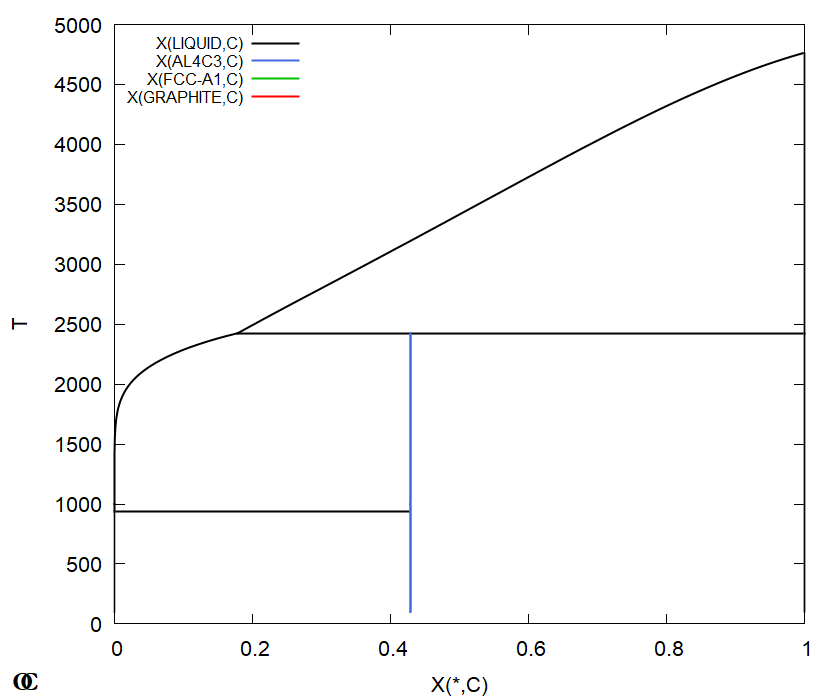
\includegraphics[width=0.45\textwidth]{AlC/AlC-PD.png}
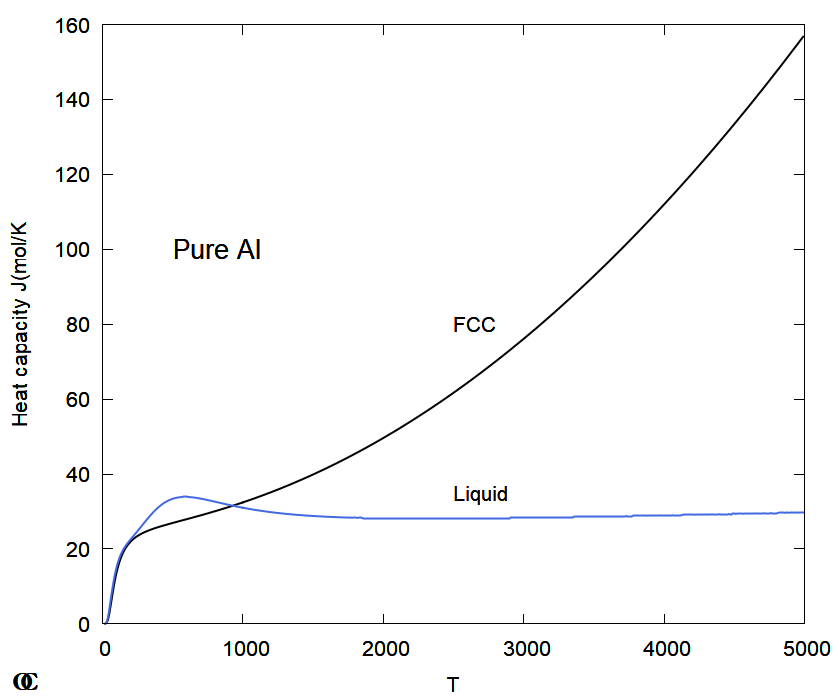
\includegraphics[width=0.45\textwidth]{AlC/Al-Cp-fcc+liquid.png}

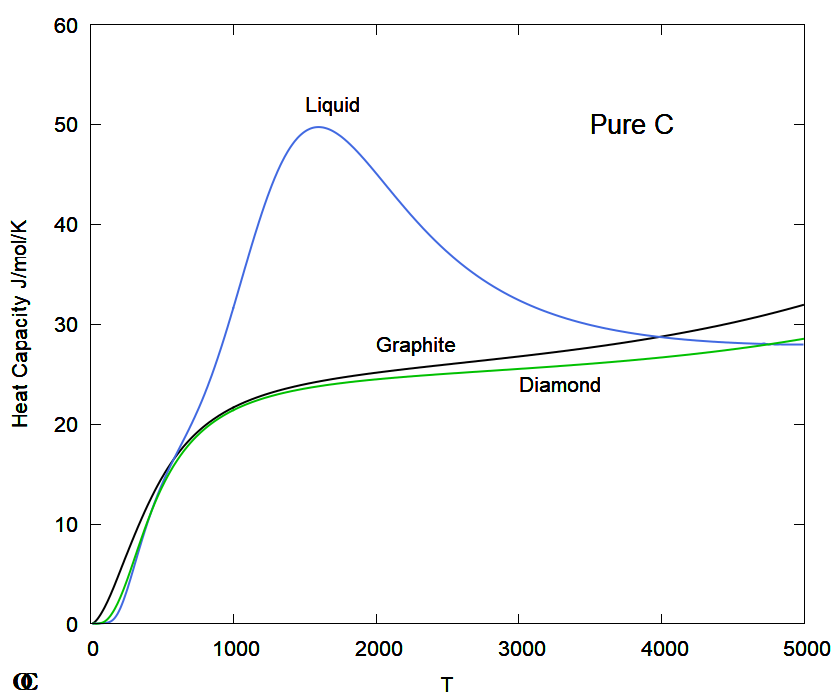
\includegraphics[width=0.45\textwidth]{AlC/C-Cp-liquid+graphite+diamond.png}
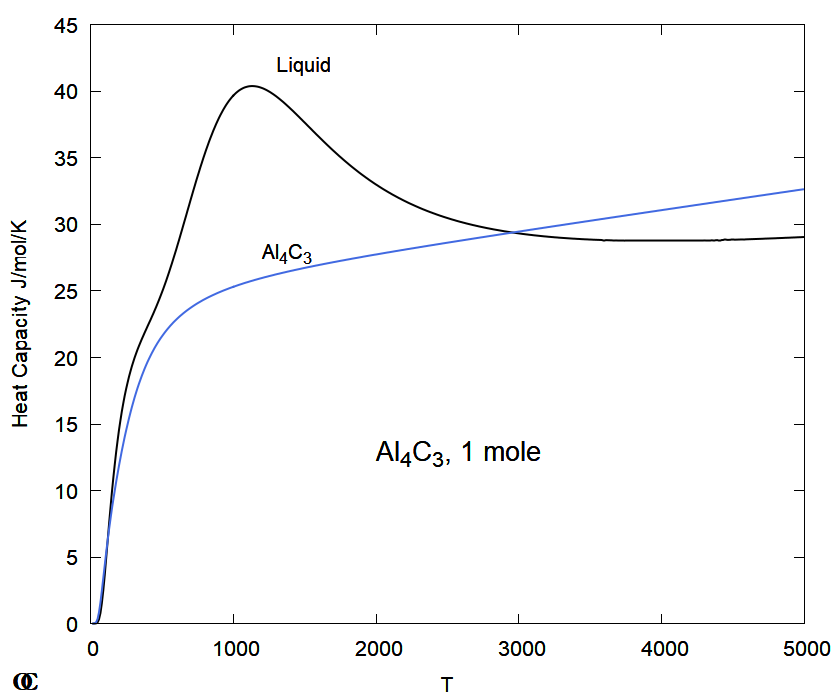
\includegraphics[width=0.45\textwidth]{AlC/Al4C3-Cp.png}

It is nice to be able to extrapolate the heat capacity down to $T=0$~K
but I propose we set the low $T$ limit at 10~K.  The rapidly
increasing heat capacity for the extrapolated metastable FCC phase
requires the EEC model to prevent the FCC to become stable at high $T$.

Adding thermal vacancies to model the increase of the heat capacity of
FCC-Al just before melting may supress the increase of the
extrapolated heat capacity but reguires some extra parameters.

\newpage

\subsection{The Al-Li system with separated disordered FCC and BCC phases
  and with these integrated in the ordered phases}

The first version in section~\ref{sec:alli1} has been generated using
a TDB file where the disordered part of the 4 sublattice FCC and BCC
phases has been described by separate phases A1\_FCC and A2\_BCC.  In
the {\bf DisorderedPart} tag this is indicated by the {\em Disordered}
attribute.  This is the way this feature is implemented in TC.  The
{\bf CrystalStructure} tag has no direct influence on the
thermodynamic calculations but if provided should be stored internally
and be provided as information to an application software and written
on any XTDB file generated by the software.

The second version in section~\ref{sec:alli2} has been generated by OC
and in OC there are no A1\_FCC or A2\_BCC phases because they are
integrated as ``disordered parts'' of the ordered phases.  Thus the
{\bf DisorderedPart} tag in the XTDB file has no no attribute {\em
  Disordered} and the parameters have a suffix ``D'' and no
sublattices for the ordering.

Both XTDB files have the same information but reflect the way the
different software handle the disordered part.  There should be
problem using slightly different ways to provide the thermodynamic
data on the XTDB files.  Each software can read the data and use its
own way to store the data and it should also implement ways to write
XTDB files in such a way that other software can read them.  It is
important that the software developers document their XTDB format to
allow other software to read their database files.

\subsubsection{The Al-Li system with ordering and crystal structures}\label{sec:alli1}

\begin{verbatim}
<Database version="0.0.1">
  <XTDB Version="0.0.3" Software="Manual" Date="2023.10.10" Signature="Bengt Hallstedt" />
  <Defaults LowT="298.15" HighT="6000" Elements="Va" />
  <DatabaseInfo>
    Database for Al-Li from B. Hallstedt and O. Kim 2007.
	B. Hallstedt, O. Kim, Int. J. Mater. Res., 98, 961-69(2007)
	Including 4-SL ordering models for fcc and bcc.
	
    Dataset created 2009.06.07 by Bengt Hallstedt.
    2016.10.22: Condensed version using option F and B.
    2020.12.20: Modified for use with GES6.
    2023.04.11: Corrected number of interstitial sites in BCC_4SL.
  </DatabaseInfo>

  <Element Id="Va" Refstate="Vacuum" Mass="0.0" H298="0.0" S298="0.0" />
  <Element Id="Al" Refstate="FCC_A1" Mass="26.98154" H298="4540.00" S298="28.30" />
  <Element Id="Li" Refstate="BCC_A2" Mass="6.941" H298="4632.00" S298="29.12" />

<!-- Do we really need these? -->
  <Species Id="Va" Stoichiometry="Va1" />
  <Species Id="Al" Stoichiometry="Al1" />
  <Species Id="Li" Stoichiometry="Li1" />

  <TPfun Id="ZERO"      Expr="0.0;" />
  <TPfun Id="UN_ASS"    Expr="0.0;" />
  <TPfun Id="R"         Expr="8.31451;" />

  <Phase Id="LIQUID" Configuration="CEF" State="L" >
    <Sites NumberOf="1" Multiplicities="1" >
      <Constituents List="Al Li" />
    </Sites>
  </Phase>

<!-- I have added crystal structure information with suggested element and attributes -->
<!-- FCC_A1 does not order -->
  <Phase Id="FCC_A1" Configuration="CEF" State="S" >
	<CrystalStructure Prototype="Cu" PearsonSymbol="cF4" SpaceGroup="Fm-3m" />
	<CrystalStructure Prototype="NaCl" PearsonSymbol="cF8" SpaceGroup="Fm-3m" />
    <Sites NumberOf="2" Multiplicities="1 1" >
      <Constituents Sublattice="1" List="Al Li" />
      <Constituents Sublattice="2" List="Va" />
    </Sites>
    <AmendPhase Models="IHJFCC" />
  </Phase>

<!-- Disordered part of FCC_4SL, identical to FCC_A1 -->
  <Phase Id="A1_FCC" Configuration="CEF" State="S" >
	<CrystalStructure Prototype="Cu" PearsonSymbol="cF4" SpaceGroup="Fm-3m" />
	<CrystalStructure Prototype="NaCl" PearsonSymbol="cF8" SpaceGroup="Fm-3m" />
    <Sites NumberOf="2" Multiplicities="1 1" >
      <Constituents Sublattice="1" List="Al Li" />
      <Constituents Sublattice="2" List="Va" />
    </Sites>
    <AmendPhase Models="IHJFCC" />
  </Phase>

  <Phase Id="FCC_4SL" Configuration="CEF" State="S" >
	<CrystalStructure Prototype="Cu" PearsonSymbol="cF4" SpaceGroup="Fm-3m" />
	<CrystalStructure Prototype="AuCu" PearsonSymbol="tP4" SpaceGroup="P4/mmm" />
	<CrystalStructure Prototype="AuCu3" PearsonSymbol="cP4" SpaceGroup="Pm-3m" />
    <Sites NumberOf="5" Multiplicities="0.25 0.25 0.25 0.25 1" >
      <Constituents Sublattice="1" List="Al Li" />
      <Constituents Sublattice="2" List="Al Li" />
      <Constituents Sublattice="3" List="Al Li" />
      <Constituents Sublattice="4" List="Al Li" />
      <Constituents Sublattice="5" List="Va" />
    </Sites>
    <DisorderedPart Disordered="A1_FCC" Sum="4" Subtract="Y" />
    <AmendPhase Models="IHJREST FCC4PERM" />
  </Phase>

<!-- BCC_A2 does not order -->
  <Phase Id="BCC_A2" Configuration="CEF" State="S" >
	<CrystalStructure Prototype="W" PearsonSymbol="cI2" SpaceGroup="Im-3m" />
    <Sites NumberOf="2" Multiplicities="1 3" >
      <Constituents Sublattice="1" List="Al Li" />
      <Constituents Sublattice="2" List="Va" />
    </Sites>
    <AmendPhase Models="IHJBCC" />
  </Phase>

<!-- Disordered part of BCC_4SL, identical to BCC_A2 -->
  <Phase Id="A2_BCC" Configuration="CEF" State="S" >
	<CrystalStructure Prototype="W" PearsonSymbol="cI2" SpaceGroup="Im-3m" />
    <Sites NumberOf="2" Multiplicities="1 3" >
      <Constituents Sublattice="1" List="Al Li" />
      <Constituents Sublattice="2" List="Va" />
    </Sites>
    <AmendPhase Models="IHJBCC" />
  </Phase>

  <Phase Id="BCC_4SL" Configuration="CEF" State="S" >
	<CrystalStructure Prototype="W" PearsonSymbol="cI2" SpaceGroup="Im-3m" />
	<CrystalStructure Prototype="CsCl" PearsonSymbol="cP2" SpaceGroup="Pm-3m" />
	<CrystalStructure Prototype="NaTl" PearsonSymbol="cF16" SpaceGroup="Fd-3m" />
	<CrystalStructure Prototype="AlFe3" PearsonSymbol="cF16" SpaceGroup="Fm-3m" />
	<CrystalStructure Prototype="AlCu2Mn" PearsonSymbol="cF16" SpaceGroup="Fm-3m" />
    <Sites NumberOf="5" Multiplicities="0.25 0.25 0.25 0.25 3" >
      <Constituents Sublattice="1" List="Al Li" />
      <Constituents Sublattice="2" List="Al Li" />
      <Constituents Sublattice="3" List="Al Li" />
      <Constituents Sublattice="4" List="Al Li" />
      <Constituents Sublattice="5" List="Va" />
    </Sites>
    <DisorderedPart Disordered="A2_BCC" Sum="4" Subtract="Y" />
    <AmendPhase Models="IHJREST BCC4PERM" />
  </Phase>

  <Phase Id="HCP_A3" Configuration="CEF" State="S" >
	<CrystalStructure Prototype="Mg" PearsonSymbol="hP2" SpaceGroup="P6_3/mmc" />
	<CrystalStructure Prototype="NiAs" PearsonSymbol="hP4" SpaceGroup="P6_3/mmc" />
    <Sites NumberOf="2" Multiplicities="1 0.5" >
      <Constituents Sublattice="1" List="Al Li" />
      <Constituents Sublattice="2" List="Va" />
    </Sites>
    <AmendPhase Models="IHJREST" />
  </Phase>

  <Phase Id="AL2LI3" Configuration="CEF" State="S" >
	<CrystalStructure Prototype="Al2Li3" PearsonSymbol="hR5" SpaceGroup="R-3m" />
    <Sites NumberOf="2" Multiplicities="2 3" >
      <Constituents Sublattice="1" List="Al" />
      <Constituents Sublattice="2" List="Li" />
    </Sites>
  </Phase>

  <Phase Id="AL4LI9" Configuration="CEF" State="S" >
	<CrystalStructure Prototype="Al4Li9" PearsonSymbol="mC26" SpaceGroup="C2/m" />
    <Sites NumberOf="2" Multiplicities="4 9" >
      <Constituents Sublattice="1" List="Al" />
      <Constituents Sublattice="2" List="Li" />
    </Sites>
  </Phase>

<!-- Unary Al -->
  <Parameter Id="G(FCC_A1,AL:VA)"  Expr="GHSERAL;" HighT="2900"  Bibref="91Din" />
  <Parameter Id="G(A1_FCC,AL:VA)"  Expr="GHSERAL;" HighT="2900"  Bibref="91Din" />
  <Parameter Id="G(BCC_A2,AL:VA)"  Expr="GHSERAL+10083-4.813*T;" HighT="2900"  Bibref="91Din" />
  <Parameter Id="G(A2_BCC,AL:VA)"  Expr="GHSERAL+10083-4.813*T;" HighT="2900"  Bibref="91Din" />
  <Parameter Id="G(HCP_A3,AL:VA)"  Expr="GHSERAL+5481-1.8*T;" HighT="2900"  Bibref="91Din" />
  <Parameter Id="G(LIQUID,AL)"  Expr="GLIQAL;" HighT="2900"  Bibref="91Din" />

  <TPfun Id="GHSERAL" Expr="-7976.15+137.093038*T-24.3671976*T*LN(T)-0.001884662*T**2-8.77664E-07*T**3+74092*T**(-1);" HighT="700" >
    <Trange Expr="-11276.24+223.048446*T-38.5844296*T*LN(T)+0.018531982*T**2 -5.764227E-06*T**3+74092*T**(-1);" HighT="933.47" /> 
    <Trange Expr="-11278.361+188.684136*T-31.748192*T*LN(T)-1.230622E+28*T**(-9);" HighT="2900" /> 
  </TPfun>

  <TPfun Id="GLIQAL" Expr="+11005.045-11.84185*T+GHSERAL+7.9337E-20*T**7;" HighT="933.47" >
     <Trange Expr="-795.991+177.430209*T-31.748192*T*LN(T);" HighT="2900" /> 
  </TPfun>

<!-- Unary Li -->
  <Parameter Id="G(BCC_A2,LI:VA)"  LowT="200" Expr="GHSERLI;" HighT="3000"  Bibref="91Din" />
  <Parameter Id="G(A2_BCC,LI:VA)"  LowT="200" Expr="GHSERLI;" HighT="3000"  Bibref="91Din" />
  <Parameter Id="G(FCC_A1,LI:VA)"  LowT="200" Expr="GHSERLI-108+1.3*T;" HighT="3000"  Bibref="91Din" />
  <Parameter Id="G(A1_FCC,LI:VA)"  LowT="200" Expr="GHSERLI-108+1.3*T;" HighT="3000"  Bibref="91Din" />
  <Parameter Id="G(HCP_A3,AL:VA)"  LowT="200" Expr="GHSERLI-154+2*T;" HighT="3000"  Bibref="91Din" />
  <Parameter Id="G(LIQUID,LI)"  LowT="200" Expr="GLIQLI;" HighT="3000"  Bibref="91Din" />

  <TPfun Id="GHSERLI" Expr="-10583.817+217.637482*T-38.940488*T*LN(T)+0.035466931*T**2-1.9869816E-05*T**3+159994*T**(-1);" HighT="453" >
    <Trange Expr="-559579.123+10547.8799*T-1702.88865*T*LN(T)+2.25832944*T**2-5.71066077E-04*T**3+33885874*T**(-1);" HighT="500" /> 
    <Trange Expr="-9062.994+179.278285*T-31.2283718*T*LN(T)+0.002633221*T**2-4.38058E-07*T**3-102387*T**(-1);" HighT="3000" /> 
  </TPfun>

  <TPfun Id="GLIQLI" Expr="+2700.205-5.795621*T+GHSERLI;" HighT="250" >
    <Trange Expr="+12015.027-362.187078*T+61.6104424*T*LN(T)-0.182426463*T**2+6.3955671E-05*T**3-559968*T**(-1);" HighT="453" /> 
    <Trange Expr="-6057.31+172.652183*T-31.2283718*T*LN(T)+0.002633221*T**2-4.38058E-07*T**3-102387*T**(-1);" HighT="500" /> 
    <Trange Expr="+3005.684-6.626102*T+GHSERLI;" HighT="3000" /> 
  </TPfun>

<!-- Binary Al-Li -->
  <Parameter Id="G(LIQUID,AL,LI;0)"  Expr="-44200+20.6*T;" Bibref="07Hal" />
  <Parameter Id="G(LIQUID,AL,LI;1)"  Expr="+13600-5.3*T;" Bibref="07Hal" />
  <Parameter Id="G(LIQUID,AL,LI;2)"  Expr="+14200;" Bibref="07Hal" />
  <Parameter Id="G(LIQUID,AL,LI;3)"  Expr="-12100;" Bibref="07Hal" />
  <Parameter Id="G(LIQUID,AL,LI;4)"  Expr="-7100;" Bibref="07Hal" />

  <Parameter Id="G(FCC_A1,AL,LI:VA;0)"  Expr="+LDF0ALLI;" Bibref="07Hal" />
  <Parameter Id="G(FCC_A1,AL,LI:VA;1)"  Expr="+LDF1ALLI;" Bibref="07Hal" />
  <Parameter Id="G(FCC_A1,AL,LI:VA;2)"  Expr="+LDF2ALLI;" Bibref="07Hal" />

  <Parameter Id="G(A1_FCC,AL,LI:VA;0)"  Expr="+LDF0ALLI;" Bibref="07Hal" />
  <Parameter Id="G(A1_FCC,AL,LI:VA;1)"  Expr="+LDF1ALLI;" Bibref="07Hal" />
  <Parameter Id="G(A1_FCC,AL,LI:VA;2)"  Expr="+LDF2ALLI;" Bibref="07Hal" />

  <Parameter Id="G(BCC_A2,AL,LI:VA;0)"  Expr="+LDB0ALLI;" Bibref="07Hal" />
  <Parameter Id="G(BCC_A2,AL,LI:VA;1)"  Expr="+LDB1ALLI;" Bibref="07Hal" />
  <Parameter Id="G(BCC_A2,AL,LI:VA;2)"  Expr="+LDB2ALLI;" Bibref="07Hal" />

  <Parameter Id="G(A2_BCC,AL,LI:VA;0)"  Expr="+LDB0ALLI;" Bibref="07Hal" />
  <Parameter Id="G(A2_BCC,AL,LI:VA;1)"  Expr="+LDB1ALLI;" Bibref="07Hal" />
  <Parameter Id="G(A2_BCC,AL,LI:VA;2)"  Expr="+LDB2ALLI;" Bibref="07Hal" />

  <Parameter Id="G(FCC_4SL,AL:AL:AL:LI:VA)"  Expr="+GFAL3LI;" Bibref="07Hal" />
  <Parameter Id="G(FCC_4SL,AL:AL:LI:LI:VA)"  Expr="+GFALLI2;" Bibref="07Hal" />
  <Parameter Id="G(FCC_4SL,AL:LI:LI:LI:VA)"  Expr="+GFALLI3;" Bibref="07Hal" />
  <Parameter Id="G(FCC_4SL,AL,LI:*:*:*:VA;0)"  Expr="+L0FALLI;" Bibref="07Hal" />
  <Parameter Id="G(FCC_4SL,AL,LI:*:*:*:VA;1)"  Expr="+L1FALLI;" Bibref="07Hal" />
  <Parameter Id="G(FCC_4SL,AL,LI:*:*:*:VA;2)"  Expr="+L2FALLI;" Bibref="07Hal" />
  <Parameter Id="G(FCC_4SL,AL,LI:AL,LI:*:*:VA;0)"  Expr="+SFALLI;" Bibref="07Hal" />

  <Parameter Id="G(BCC_4SL,AL:AL:AL:LI:VA)"  Expr="+GBAL3LI;" Bibref="07Hal" />
  <Parameter Id="G(BCC_4SL,AL:AL:LI:LI:VA)"  Expr="+GB2ALLI;" Bibref="07Hal" />
  <Parameter Id="G(BCC_4SL,AL:LI:AL:LI:VA)"  Expr="+GB2ALLI;" Bibref="07Hal" />
  <Parameter Id="G(BCC_4SL,AL:LI:LI:LI:VA)"  Expr="+GBALLI3;" Bibref="07Hal" />
  <Parameter Id="G(BCC_4SL,AL,LI:*:*:*:VA;0)"  Expr="+L0BALLI;" Bibref="07Hal" />
  <Parameter Id="G(BCC_4SL,AL,LI:*:*:*:VA;1)"  Expr="+L1BALLI;" Bibref="07Hal" />
  <Parameter Id="G(BCC_4SL,AL,LI:*:*:*:VA;2)"  Expr="+L2BALLI;" Bibref="07Hal" />
  <Parameter Id="G(BCC_4SL,AL,LI:AL,LI:*:*:VA;0)"  Expr="+SB1ALLI;" Bibref="07Hal" />
  <Parameter Id="G(BCC_4SL,AL,LI:*:AL,LI:*:VA;0)"  Expr="+SB2ALLI;" Bibref="07Hal"  />
  
  <Parameter Id="G(AL2LI3,AL:LI)"  Expr="+2*GHSERAL+3*GHSERLI-93990+34.5*T;" Bibref="07Hal" />
  <Parameter Id="G(AL4LI),AL:LI)"  Expr="+4*GHSERAL+9*GHSERLI-193780+71.7*T;" Bibref="07Hal" />

<!-- metastable -->
  <Parameter Id="G(HCP_A3,AL,LI:VA;0)"  Expr="-27000+8*T;" Bibref="98Sau2" />

  <TPfun Id="UFALLI" Expr="-3270+1.96*T;" />
  <TPfun Id="L0FALLI" Expr="+2960-1.56*T;" />
  <TPfun Id="L2FALLI" Expr="0;" />
  <TPfun Id="L2FALLI" Expr="0;" />
  <TPfun Id="GFAL3LI" Expr="+3*UFALLI+1750-4.7*T;" />
  <TPfun Id="GFAL2LI2" Expr="+4*UFALLI;" />
  <TPfun Id="GFALLI3" Expr="+3*UFALLI+4900;" />
  <TPfun Id="SFALLI" Expr="+UFALLI;" />
  <TPfun Id="LDF0ALLI" Expr="+GFAL3LI+1.5*GFAL2LI2+GFALLI3+1.5*SFALLI+4*L0FALLI;" />
  <TPfun Id="LDF1ALLI" Expr="+2*GFAL3LI-2*GFALLI3+4*L1FALLI;" />
  <TPfun Id="LDF2ALLI" Expr="+GFAL3LI-1.5*GFAL2LI2+GFALLI3-1.5*SFALLI+4*L2FALLI;" />

  <TPfun Id="UB1ALLI" Expr="-3360+1.8*T;" />
  <TPfun Id="UB2ALLI" Expr="-4230+1.86*T;" />
  <TPfun Id="L0BALLI" Expr="0;" />
  <TPfun Id="L2BALLI" Expr="0;" />
  <TPfun Id="L2BALLI" Expr="0;" />
  <TPfun Id="GBAL3LI" Expr="+2*UB1ALLI+1.5*UB2ALLI+3700;" />
  <TPfun Id="GB2ALLI" Expr="+4*UB1ALLI;" />
  <TPfun Id="GB32ALLI" Expr="+2*UB1ALLI+3*UB2ALLI;" />
  <TPfun Id="GBALLI3" Expr="+2*UB1ALLI+1.5*UB2ALLI+3250;" />
  <TPfun Id="SB1ALLI" Expr="+15000;" />
  <TPfun Id="SB2ALLI" Expr="+15000;" />
  <TPfun Id="LDB0ALLI" Expr="+GBAL3LI+0.5*GB2ALLI+GB32ALLI+GBALLI3+4*L0BALLI;" />
  <TPfun Id="LDB1ALLI" Expr="+2*GBAL3LI-2*GBALLI3+4*L1BALLI;" />
  <TPfun Id="LDB2ALLI" Expr="+GBAL3LI-0.5*GB2ALLI-GB32ALLI+GBALLI3+4*L2BALLI;" />

  <Bibliography>
    <Bibitem Id="91Din" Text="A.T. Dinsdale, Calphad, 15, 317-425(1991)." />
    <Bibitem Id="98Sau2" Text="N. Saunders, COST 507, Final report round 2, 1998; Al-Li" />
    <Bibitem Id="07Hal" Text="B. Hallstedt, O. Kim, Int. J. Mater. Res., 98, 961-69(2007); Al-Li" />
  </Bibliography> 

</Database>
\end{verbatim}

\subsubsection{The Al-Li system with the disordered parameters
  integrated in the ordered phases}\label{sec:alli2}

This XTDB file for Al-Ni is generated from OC with the
``DisorderedPart'' integrated in the ordered FCC and BCC phases.  Note
the suffix ``D'' and the reduced number of sublattices for the Gibbs
energy parameters in the disordered part.

In this listing all {\bf TPfun} tags are in the beginning, the {\bf
  CrystalStructure} tag is missing and the parameters for all phases
listed together at the end.  The list of parameters has been edited
manually and may contain some errors.

\begin{verbatim}
<Database version="0.0.3">
  <metadata>
    <writer Software="OpenCalphad  6.067" Date="2023-10-15" />
  </metadata>
  <Defaults LowT="298.15" HighT="6000" Bibref="U.N. Known" Elements="VA /-" />
  <Element Id="AL" Refstate="FCC_A1" Mass="2.698154E+01" H298="4.540000E+03" S298="2.830000E+01" />
  <Element Id="LI" Refstate="BCC_A2" Mass="6.941000E+00" H298="4.632000E+03" S298="2.912000E+01" />
  <Species Id="VA" Stoichiometry="VA" />
  <Species Id="AL" Stoichiometry="AL" />
  <Species Id="LI" Stoichiometry="LI" />
  <TPfun Id="R"     Expr="8.31451;" />
  <TPfun Id="RTLNP" Expr="R*T*LN(1.0E-5)*P);" />
  <TPfun Id="GHSERAL" Expr=" -7976.15+137.093038*T-24.3671976*T*LN(+T)-.001884662*T**2-8.77664E-07*T**3+74092*T**(-1);" HighT="700" >
    <Trange Expr="-11276.24+223.048446*T-38.5844296*T*LN(+T)+.018531982*T**2-5.764227E-06*T**3+74092*T**(-1);" HighT="933.47" />
    <Trange Expr="-11278.378+188.684153*T-31.748192*T*LN(+T)-1.230524E+28*T**(-9);" HighT="2900" /> 
  </TPfun>
  <TPfun Id="GLIQAL" Expr=" +11005.029-11.841867*T+GHSERAL+7.9337E-20*T**7;" HighT="933.47" >
    <Trange Expr="-795.996+177.430178*T-31.748192*T*LN(+T);" HighT="2900" /> 
  </TPfun>
  <TPfun Id="GHSERLI" LowT="200" Expr=" -10583.817+217.637482*T-38.940488*T*LN(+T)+.035466931*T**2-1.9869816E-05*T**3+159994*T**(-1);" HighT="453.6" >
    <Trange Expr="-559579.123+10547.8799*T-1702.88865*T*LN(+T)+2.25832944*T**2-.000571066077*T**3+33885874*T**(-1);" HighT="500" />
    <Trange Expr="-9062.994+179.278285*T-31.2283718*T*LN(+T)+.002633221*T**2-4.38058E-07*T**3-102387*T**(-1);" HighT="3000" /> 
  </TPfun>
  <TPfun Id="GLIQLI" LowT="200" Expr=" +2700.205-5.795621*T+GHSERLI;" HighT="250" >
    <Trange Expr="+12015.027-362.187078*T+61.6104424*T*LN(+T)-0.182426463*T**2+6.3955671E-05*T**3-559968*T**(-1);" HighT="453.6" />
    <Trange Expr="-6057.31+172.652183*T-31.2283718*T*LN(+T)+.002633221*T**2-4.38058E-07*T**3-102387*T**(-1);" HighT="500" />
    <Trange Expr="+3005.684-6.626102*T+GHSERLI;" HighT="3000" /> 
  </TPfun>
  <TPfun Id="LDF0ALLI" Expr=" +GFAL3LI+1.5*GFAL2LI2+GFALLI3+1.5*SFALLI+4*L0FALLI;" /> 
  <TPfun Id="LDF1ALLI" Expr=" +2*GFAL3LI-2*GFALLI3+4*L1FALLI;" /> 
  <TPfun Id="LDF2ALLI" Expr=" +GFAL3LI-1.5*GFAL2LI2+GFALLI3-1.5*SFALLI+4*L2FALLI;" /> 
  <TPfun Id="LDB0ALLI" Expr=" +GBAL3LI+0.5*GB2ALLI+GB32ALLI+GBALLI3+4*L0BALLI;" /> 
  <TPfun Id="LDB1ALLI" Expr=" +2*GBAL3LI-2*GBALLI3+4*L1BALLI;" /> 
  <TPfun Id="LDB2ALLI" Expr=" +GBAL3LI-0.5*GB2ALLI-GB32ALLI+GBALLI3+4*L2BALLI;" /> 
  <TPfun Id="GFAL3LI" Expr=" +3*UFALLI+1750-4.7*T;" /> 
  <TPfun Id="GFAL2LI2" Expr=" +4*UFALLI;" /> 
  <TPfun Id="L0FALLI" Expr=" +2960-1.56*T;" /> 
  <TPfun Id="L1FALLI" Expr=" 0;" /> 
  <TPfun Id="L2FALLI" Expr=" 0;" /> 
  <TPfun Id="SFALLI" Expr=" +UFALLI;" /> 
  <TPfun Id="GBAL3LI" Expr=" +2*UB1ALLI+1.5*UB2ALLI+3700;" /> 
  <TPfun Id="GB2ALLI" Expr=" +4*UB1ALLI;" /> 
  <TPfun Id="GBALLI3" Expr=" +2*UB1ALLI+1.5*UB2ALLI+3250;" /> 
  <TPfun Id="L0BALLI" Expr=" 0;" /> 
  <TPfun Id="L1BALLI" Expr=" 0;" /> 
  <TPfun Id="L2BALLI" Expr=" 0;" /> 
  <TPfun Id="SB1ALLI" Expr=" +15000;" /> 
  <TPfun Id="UFALLI" Expr=" -3270+1.96*T;" /> 
  <TPfun Id="GFALLI3" Expr=" +3*UFALLI+4900;" /> 
  <TPfun Id="UB1ALLI" Expr=" -3360+1.8*T;" /> 
  <TPfun Id="UB2ALLI" Expr=" -4230+1.86*T;" /> 
  <TPfun Id="GB32ALLI" Expr=" +2*UB1ALLI+3*UB2ALLI;" /> 
  <Phase Id="LIQUID" Configuration="CEF" State="L" >
    <Sites NumberOf="1" Multiplicities="1" >
      <Constituents List="AL LI" />
    </Sites>
  </Phase>
  <Phase Id="AL2LI3" Configuration="CEF" State="S" >
    <Sites NumberOf="2" Multiplicities="2 3" >
      <Constituents Sublattice="1" List="AL" />
      <Constituents Sublattice="2" List="LI" />
    </Sites>
  </Phase>
  <Phase Id="AL4LI9" Configuration="CEF" State="S" >
    <Sites NumberOf="2" Multiplicities="4 9" >
      <Constituents Sublattice="1" List="AL" />
      <Constituents Sublattice="2" List="LI" />
    </Sites>
  </Phase>
  <Phase Id="BCC_A2" Configuration="CEF" State="S" >
    <Sites NumberOf="2" Multiplicities="1 3" >
      <Constituents Sublattice="1" List="AL LI" />
      <Constituents Sublattice="2" List="VA" />
    </Sites>
  </Phase>
  <Phase Id="HCP_A3" Configuration="CEF" State="S" >
    <Sites NumberOf="2" Multiplicities="1 0.5" >
      <Constituents Sublattice="1" List="AL LI" />
      <Constituents Sublattice="2" List="VA" />
    </Sites>
  </Phase>
  <Phase Id="BD3_BCC" Configuration="CEF" State="S" >
    <Sites NumberOf="5" Multiplicities="0.25 0.25 0.25 0.25 1" >
      <Constituents Sublattice="1" List="AL LI" />
      <Constituents Sublattice="2" List="AL LI" />
      <Constituents Sublattice="3" List="AL LI" />
      <Constituents Sublattice="4" List="AL LI" />
      <Constituents Sublattice="5" List="VA" />
    </Sites>
    <DisorderedPart Subtract="Y" Sum="4" />
    <AmendPhase Models="BCC4PERM" />
  </Phase>
  <Phase Id="FCC_A1" Configuration="CEF" State="S" >
    <Sites NumberOf="2" Multiplicities="1 1" >
      <Constituents Sublattice="1" List="AL LI" />
      <Constituents Sublattice="2" List="VA" />
    </Sites>
  </Phase>
  <Phase Id="L102_FCC" Configuration="CEF" State="S" >
    <Sites NumberOf="5" Multiplicities="0.25 0.25 0.25 0.25 1" >
      <Constituents Sublattice="1" List="AL LI" />
      <Constituents Sublattice="2" List="AL LI" />
      <Constituents Sublattice="3" List="AL LI" />
      <Constituents Sublattice="4" List="AL LI" />
      <Constituents Sublattice="5" List="VA" />
    </Sites>
    <DisorderedPart Subtract="Y" Sum="4" />
    <AmendPhase Models="FCC4PERM" />
  </Phase>
  <Parameter Id="G(LIQUID,AL;0)"  Expr=" +GLIQAL;" HighT="2900"  Bibref="91DIN" />
  <Parameter Id="G(LIQUID,LI;0)"  LowT="200" Expr=" +GLIQLI;" HighT="3000"  Bibref="91DIN" />
  <Parameter Id="G(LIQUID,AL,LI;0)"  Expr=" -44200+20.6*T;"  Bibref="07HAL" />
  <Parameter Id="G(LIQUID,AL,LI;1)"  Expr=" +13600-5.3*T;"  Bibref="07HAL" />
  <Parameter Id="G(LIQUID,AL,LI;2)"  Expr=" +14200;"  Bibref="07HAL" />
  <Parameter Id="G(LIQUID,AL,LI;3)"  Expr=" -12100;"  Bibref="07HAL" />
  <Parameter Id="G(LIQUID,AL,LI;4)"  Expr=" -7100;"  Bibref="07HAL" />

  <Parameter Id="G(AL2LI3,AL:LI;0)"  Expr=" +2*GHSERAL+3*GHSERLI-93990+34.5*T;"  Bibref="07HAL" />
  <Parameter Id="G(AL4LI9,AL:LI;0)"  Expr=" +4*GHSERAL+9*GHSERLI-193780+71.7*T;"  Bibref="07HAL" />

  <Parameter Id="G(BCC_A2,AL:VA;0)"  Expr=" +GHSERAL+10083-4.813*T;" HighT="2900"  Bibref="91DIN" />
  <Parameter Id="G(BCC_A2,LI:VA;0)"  LowT="200" Expr=" +GHSERLI;" HighT="3000"  Bibref="91DIN" />
  <Parameter Id="G(BCC_A2,AL,LI:VA;0)"  Expr=" +LDB0ALLI;"  Bibref="07HAL" />
  <Parameter Id="G(BCC_A2,AL,LI:VA;1)"  Expr=" +LDB1ALLI;"  Bibref="07HAL" />
  <Parameter Id="G(BCC_A2,AL,LI:VA;2)"  Expr=" +LDB2ALLI;"  Bibref="07HAL" />
  <Parameter Id="G(HCP_A3,AL:VA;0)"  Expr=" +GHSERAL+5481-1.8*T;" HighT="2900"  Bibref="91DIN" />
  <Parameter Id="G(HCP_A3,LI:VA;0)"  LowT="200" Expr=" +GHSERLI-154+2*T;" HighT="3000"  Bibref="91DIN" />
  <Parameter Id="G(HCP_A3,AL,LI:VA;0)"  Expr=" -27000+8*T;"  Bibref="98SAU2" />

  <Parameter Id="G(BD3_BCC,AL:AL:AL:LI:VA;0)"  Expr=" +GBAL3LI;"  Bibref="07HAL" />
  <Parameter Id="G(BD3_BCC,AL:LI:AL:AL:VA;0)"  Expr=" +GBAL3LI;"  Bibref="07HAL" />
  <Parameter Id="G(BD3_BCC,AL:AL:LI:LI:VA;0)"  Expr=" +GB2ALLI;"  Bibref="07HAL" />
  <Parameter Id="G(BD3_BCC,LI:LI:AL:AL;VA;0)"  Expr=" +GB32ALLI;"  Bibref="07HAL" />
  <Parameter Id="G(BD3_BCC,AL:LI:AL:LI:VA;0)"  Expr=" +GBALLI3;"  Bibref="07HAL" />
  <Parameter Id="G(BD3_BCC,LI:LI:AL:LI:VA;0)"  Expr=" +GBALLI3;"  Bibref="07HAL" />
  <Parameter Id="G(BD3_BCC,AL,LI:AL,LI:*:*:VA;0)"  Expr=" +SB1ALLI;"  Bibref="07HAL" />
  <Parameter Id="G(BD3_BCC,AL,LI:*:*:*:VA;0)"  Expr=" +L0BALLI;"  Bibref="07HAL" />
  <Parameter Id="G(BD3_BCC,AL,LI:*:*:*:VA;1)"  Expr=" +L1BALLI;"  Bibref="07HAL" />
  <Parameter Id="G(BD3_BCC,AL,LI:*:*:*:VA;2)"  Expr=" +L2BALLI;"  Bibref="07HAL" />
<!-- Disordered fraction set factor:     1.0000 Sublattices:   2 with suffix D -->
  <Parameter Id="GD(BD3_BCC,AL:VA;0)"  Expr=" +GHSERAL+10083-4.813*T;" HighT="2900"  Bibref="91DIN" />
  <Parameter Id="GD(BD3_BCC,LI:VA;0)"  LowT="200" Expr=" +GHSERLI;" HighT="3000"  Bibref="91DIN" />
  <Parameter Id="GD(BD3_BCC,AL,LI:VA;0)"  Expr=" +LDB0ALLI;"  Bibref="07HAL" />
  <Parameter Id="GD(BD3_BCC,AL,LI:VA;1)"  Expr=" +LDB1ALLI;"  Bibref="07HAL" />
  <Parameter Id="GD(BD3_BCC,AL,LI:VA;2)"  Expr=" +LDB2ALLI;"  Bibref="07HAL" />

  <Parameter Id="G(FCC_A1,AL:VA;0)"  Expr=" +GHSERAL;" HighT="2900"  Bibref="91DIN" />
  <Parameter Id="G(FCC_A1,LI:VA;0)"  LowT="200" Expr=" +GHSERLI-108+1.3*T;" HighT="3000"  Bibref="91DIN" />
  <Parameter Id="G(FCC_A1,AL,LI:VA;0)"  Expr=" +LDF0ALLI;"  Bibref="07HAL" />
  <Parameter Id="G(FCC_A1,AL,LI:VA;1)"  Expr=" +LDF1ALLI;"  Bibref="07HAL" />
  <Parameter Id="G(FCC_A1,AL,LI:VA;2)"  Expr=" +LDF2ALLI;"  Bibref="07HAL" />

  <Parameter Id="G(L102_FCC,AL:AL:AL:LI:VA;0)"  Expr=" +GFAL3LI;"  Bibref="07HAL" />
  <Parameter Id="G(L102_FCC,AL:AL:LI:LI:VA;0)"  Expr=" +GFAL2LI2;"  Bibref="07HAL" />
  <Parameter Id="G(L102_FCC,AL:LI:LI:LI:VA;0)"  Expr=" +GFALLI3;"  Bibref="07HAL" />
  <Parameter Id="G(L102_FCC,*:*:AL,LI:AL,LI:VA;0)"  Expr=" +SFALLI;"  Bibref="07HAL" />
  <Parameter Id="G(L102_FCC,*:*:*:AL,LI:VA;0)"  Expr=" +L0FALLI;"  Bibref="07HAL" />
  <Parameter Id="G(L102_FCC,*:*:*:AL,LI:VA;1)"  Expr=" +L1FALLI;"  Bibref="07HAL" />
  <Parameter Id="G(L102_FCC,*:*:*:AL,LI:VA;2)"  Expr=" +L2FALLI;"  Bibref="07HAL" />
<!-- Disordered fraction set factor:     1.0000 Sublattices:   2 with suffix D-->
  <Parameter Id="GD(L102_FCC,AL:VA;0)"  Expr=" +GHSERAL;" HighT="2900"  Bibref="91DIN" />
  <Parameter Id="GD(L102_FCC,LI:VA;0)"  LowT="200" Expr=" +GHSERLI-108+1.3*T;" HighT="3000"  Bibref="91DIN" />
  <Parameter Id="GD(L102_FCC,AL,LI:VA;0)"  Expr=" +LDF0ALLI;"  Bibref="07HAL" />
  <Parameter Id="GD(L102_FCC,AL,LI:VA;1)"  Expr=" +LDF1ALLI;"  Bibref="07HAL" />
  <Parameter Id="GD(L102_FCC,AL,LI:VA;2)"  Expr=" +LDF2ALLI;"  Bibref="07HAL" />
  <Bibliograpy>
    <Bibitem Id="91DIN" Text="A.T. Dinsdale, Calphad, 15, 317-425(1991)." /> 
    <Bibitem Id="07HAL" Text="B. Hallstedt, O. Kim, Int. J. Mater. Res., 98, 961-69(2007); Al-Li" /> 
    <Bibitem Id="98SAU2" Text="N. Saunders, COST 507, Final report round 2, 1998; Al-Li" /> 
    <Bibitem Id="Default" Text="U.N. Known" /> 
  </Bibliograpy>


</Database>
\end{verbatim}

\end{appendices}
\end{document}

